\documentclass[11pt,a4paper]{article}

% , -- packages , --
\usepackage[utf8]{inputenc}
\usepackage[T1]{fontenc}
\usepackage{lmodern}
\usepackage{microtype}
\usepackage[hidelinks]{hyperref}
\usepackage{url}
\usepackage{amsmath,amssymb}
\usepackage{booktabs}
\usepackage{graphicx}
\usepackage{xcolor}
\usepackage{listings}
\usepackage{cite}
\usepackage{natbib}
\usepackage[margin=1in]{geometry}
\usepackage{enumitem}
\usepackage{siunitx}
\usepackage{xspace}

% , -- listing style , --
\lstset{
  basicstyle=\ttfamily\footnotesize,
  breaklines=true,
  columns=fullflexible,
  frame=single,
  xleftmargin=1em,
  xrightmargin=1em,
  showstringspaces=false,
}

\newcommand{\tool}{\textsc{cukereuse}\xspace}

% Allow LaTeX extra flexibility on otherwise-overfull lines so that long
% hyphenated compounds (e.g. "permissively-licensed", "step-duplication",
% "behaviour-catalogue") stay within the right margin rather than protruding.
\emergencystretch=3em

% Custom hyphenation patterns for compound words that LaTeX's default
% dictionary does not split well.
\hyphenation{
  per-mis-sive-ly per-mis-sive-ly-licensed
  co-py-left co-py-left-licensed
  para-phrase-robust para-phrase para-phrases
  step-dup-li-ca-tion dup-li-ca-tion
  be-ha-viour be-ha-viour-driven
  script-ing-lan-guage
  script-ing
}

\title{Finding Duplicates in 1.1M BDD Steps: \tool, a Paraphrase-Robust Static Detector for Cucumber and Gherkin}

\author{%
  Ali Hassaan Mughal\\
  Independent Researcher\\
  Applied MBA (Data Analytics), Texas Wesleyan University, USA\\
  \texttt{alihassaanmughal.work@gmail.com}\\
  ORCID: \href{https://orcid.org/0000-0002-0724-9197}{0000-0002-0724-9197}
  \and
  Noor Fatima\\
  Independent Researcher\\
  B.E. Computer Engineering, National University of Sciences and
  Technology (NUST), Pakistan\\
  \texttt{noorfatima.ce@gmail.com}
  \and
  Muhammad Bilal\\
  Independent Researcher\\
  M.Sc. Management, Technical University of Munich, Germany\\
  \texttt{m.bilal@tum.de}\\
  ORCID: \href{https://orcid.org/0000-0003-4106-0256}{0000-0003-4106-0256}
}

\date{April 2026}

\begin{document}
\maketitle

\begin{abstract}
Behaviour-Driven Development (BDD) suites accumulate step-text
duplication whose maintenance cost is established in prior work.
Existing detection techniques require running the tests (Binamungu
et al., 2018-2023) or are confined to a single organisation
(Irshad et al., 2020-2022), leaving a gap: a purely static,
paraphrase-robust, step-level detector usable on any repository.
We fill the gap with \tool, an open-source Python CLI combining
exact hashing, Levenshtein ratio, and sentence-transformer
embeddings in a layered pipeline, released alongside an empirical
corpus of 347 public GitHub repositories, 23{,}667 parsed
\texttt{.feature} files, and 1{,}113{,}616 Gherkin steps. The
step-weighted exact-duplicate rate is 80.2\,\%; the
median-repository rate is 58.6\,\% (Spearman $\rho = 0.51$ with
size). The top hybrid cluster groups 20.7k occurrences across 2.2k
files. Against 1{,}020 pairs manually labelled by the three authors
under a released rubric (inter-annotator Fleiss' $\kappa = 0.84$ on
a 60-pair overlap), we report precision, recall, and F$_1$ with
bootstrap 95\,\% CIs under two protocols: the primary rubric and a
score-free second-pass relabelling. The strongest honest pair-level
number is near-exact at F$_1 = 0.822$ on score-free labels; the
primary-rubric semantic F$_1 = 0.906$ is inflated by a
stratification artefact that pins recall at 1.000. Lexical
baselines (SourcererCC-style, NiCad-style) reach primary
F$_1 = 0.761$ and $0.799$. The paper also presents a CDN-structured
critique of Gherkin (Cognitive Dimensions of Notations); eight of
fourteen dimensions are rated problematic or unsupported. The tool,
corpus, labelled pairs, rubric, and pipeline are released under
permissive licences.
\end{abstract}

\vspace{1ex}
\noindent\textbf{Keywords:} Behaviour-Driven Development; BDD;
Cucumber; Gherkin; duplicate detection; clone detection;
paraphrase-robust matching; static analysis; sentence-transformer;
semantic similarity; neural clone detection; test automation;
AI-assisted testing; LLM evaluation; agentic AI;
empirical software engineering; mining software
repositories; cognitive dimensions of notations; software
maintenance; test refactoring; test specification; software quality.

\section{Introduction}
\label{sec:introduction}

Gherkin, the near-English notation used by Cucumber, Behat, SpecFlow,
pytest-bdd, behave, and related Behaviour-Driven Development (BDD)
frameworks \citep{north2006bdd,wynne2017cucumber}, is deployed at
considerable scale in industry. Our own survey of public GitHub places
approximately 55{,}000 \texttt{.feature} files in indexable repositories;
the sampled subset we assemble in this paper comprises 347 active
projects, approximately 23.7k parsed feature files, and over 1.1M individual steps
(Section~\ref{sec:corpus}). Across that corpus, \emph{more than four out
of every five steps are byte-identical duplicates of another step in the
same corpus}. When paraphrase-robust matching is applied, matching
\texttt{the response status is 200 OK} with \texttt{status 200} and with
\texttt{the response status should be "200"}, the most-repeated canonical
step phrasing appears 20{,}737 times across 2{,}245 distinct files.

Duplication of this shape is not merely a hygiene issue, and this paper
does not treat it as one. Prior BDD-quality work establishes the cost
independently of our measurement: \citet{binamungu2018vst} identify
scenario-level duplication as a first-class quality defect in industrial
BDD suites and argue that duplicate steps bound to divergent glue code
silently drift in production behaviour; \citet{oliveira2017quality} and
\citet{oliveira2019quality} catalogue practitioner-reported quality
concerns in BDD scenarios, with duplication and paraphrase inconsistency
recurring among the top three; \citet{irshad2021jss} and
\citet{irshad2022ist} quantify the effort impact of step reuse inside
Ericsson's BDD suite over multiple years. When two step-text phrasings
bind to \emph{different} step-definition functions in the glue code,
the Gherkin notation silently hides a dependency: two scenarios that
look equivalent on the page execute different logic in production.
The same step text bound to two different definitions, a pattern we
observe in multiple projects in our corpus, produces silent test drift
that the BDD runner cannot diagnose. Our contribution is therefore a
detection layer for a cost that prior work has already established as
real; whether that detection is actionable depends on the maintainer's
context, and §\ref{sec:discussion} reads the findings in that light.

Three prior bodies of work occupy the adjacent territory. Binamungu et
al.\ detect duplicate \emph{scenarios} via dynamic execution tracing
\citep{binamungu2018vst,binamungu2018saner,binamungu2020xp,binamungu2020phd};
their technique requires the tests to actually run, which is infeasible
for cross-repository analysis of the scale we target. Irshad et al.\
apply Normalised Compression Distance at industrial scale within a
single organisation \citep{irshad2020ease,irshad2021jss,irshad2022ist};
their technique is neither neural nor step-level. A Manchester MSc
\citep{suan2015msc} combined textual and AST-based similarity on Gherkin
but remained unpublished. No prior work applies modern sentence
embeddings to Cucumber steps or performs duplicate detection at
step-text level across a published cross-repository corpus.

\subsection*{Contributions}

\begin{enumerate}[leftmargin=2em]
  \item A purely static, paraphrase-robust, step-level duplicate
        detector for Gherkin, comprising four strategies (exact hash,
        normalised Levenshtein, sentence-embedding cosine, and
        hybrid) with empirically-calibrated decision thresholds. The
        implementation is released as an open-source Python CLI under
        the Apache 2.0 licence and is \texttt{pip}-installable.
  \item A cross-organisational empirical corpus of Gherkin
        \texttt{.feature} files (Table~\ref{tab:corpus-compare}): 347
        public GitHub repositories, 23{,}667 parsed
        \texttt{.feature} files, 1{,}113{,}616 steps, with SPDX
        license metadata per repository and a pointer-based
        reproducibility scheme that complies with the copyleft licence
        of repositories we cannot directly redistribute.
  \item A Gebru-style datasheet for the corpus \citep{gebru2021datasheets}.
  \item A CDN-structured (Cognitive Dimensions of Notations)
        critique of Gherkin, grounding each of the 14 dimensions in
        concrete corpus examples. We frame it as a critique rather
        than a canonical CDN study because the ratings are author
        assessments rather than the outcome of questionnaire-based
        elicitation from users or designers, which is the methodology
        canonical CDN contributions typically follow; §\ref{sec:cdn}
        discloses this limitation explicitly.
  \item An empirical threshold-calibration study on 1{,}020 labelled pairs
        stratified across cosine-similarity bands, reporting precision,
        recall, and F$_1$ with bootstrap 95\,\% confidence intervals per
        strategy. Two lexical baselines representing classical
        token-based clone detection (SourcererCC-style and NiCad-style)
        are run on the same benchmark for direct comparison. A
        score-free second-pass relabelling, that uses no cosine or
        Levenshtein values in its labelling criteria, quantifies the
        circularity cost of the primary rubric's score-based positive
        rules.
  \item A methodological finding: the threshold that maximises pair-level
        F$_1$ (\(\approx 0.55\) Levenshtein ratio) differs sharply from
        the threshold that prevents transitive single-linkage chaining
        in cluster-level analysis (\(\approx 0.92\)), with direct
        consequences for downstream use.
\end{enumerate}

\subsection*{Research questions}

The paper is organised around four research questions:

\begin{description}[leftmargin=2.2em,labelindent=0em,style=nextline]
\item[RQ1 (prevalence).] At what rate does step-text duplication
occur in real cross-organisational BDD suites, and does the rate
depend on licence class or repository size?
\item[RQ2 (detection quality).] How well do a layered static
pipeline (exact, near-exact, semantic, hybrid) and two classical
lexical baselines (SourcererCC-style token Jaccard, NiCad-style
TF-IDF character $n$-gram cosine) classify pairs against an
author-labelled benchmark, and what is the effect size of each
strategy's advantage?
\item[RQ3 (methodological coupling).] How much of the reported
F$_1$ reflects circularity between score-based labelling rules and
score-based detectors, and what is the detector's performance
against a score-free relabelling of the same pair set?
\item[RQ4 (cognitive fit).] When Gherkin is evaluated against the
fourteen Cognitive Dimensions of Notations, which dimensions are
supported and which are problematic, and what concrete tool
interventions do the problematic dimensions motivate?
\end{description}

Section~\ref{sec:corpus} addresses RQ1 (headline rate, licence
stratification, size analysis), Section~\ref{sec:evaluation}
addresses RQ2 and RQ3 (calibration, baselines, score-free
relabelling), and Section~\ref{sec:cdn} addresses RQ4.

We frame our contribution as \emph{orthogonal} to execution-based
scenario-duplicate detection \citep{binamungu2018vst}: the two
techniques target different analysis levels (step-text vocabulary
clustering versus scenario-level behavioural equivalence) and a
production BDD toolchain could productively deploy both. Our target
audience is the maintainer of a BDD suite that has grown beyond one
team's cognitive span.

The present paper continues a line of work on automated software
testing and test-artefact quality that the author has contributed
to over several prior publications. \citet{mughal2024bdd}
implemented dynamic scenario re-usability in the Cucumber
Java framework, demonstrated a VSCode extension offering step-
definition auto-completion to test authors, and reported
integration with a Jenkins-plus-Maven continuous-delivery
pipeline. \citet{mughal2025rlagent} developed an autonomous
reinforcement-learning agent that dynamically generates and
refines BDD test scenarios for web-UI testing, with a state
representation, action space, and reward mechanism that guide
exploration of UI states and report improvements in defect
detection and test coverage on open-source web applications.
\citet{mughal2026networklayer} moves the testing perspective
one layer down the stack, capturing production HTTP traffic
from 18 real-world websites via browser instrumentation and
applying eight heuristic anti-pattern detectors to derive a
composite quality score. Read together, the three papers step
outward from single-framework tooling (2024) to dynamic agent-
based scenario generation (2025) to production-level HTTP
traffic analysis (2026). Cukereuse fills a complementary slot:
\emph{static, corpus-scale analysis of BDD step text}, the one
dimension of test-artefact quality the three prior papers do
not themselves tackle. In the Discussion
(Section~\ref{sec:discussion:integration}) and Future Work
(Section~\ref{sec:future}) sections we identify concrete
integration points with each of the prior papers where the
duplicate-detection output of the present work is directly
useful.

Section~\ref{sec:background} surveys BDD, clone detection, and CDN.
Section~\ref{sec:related} positions our work against prior art.
Section~\ref{sec:cdn} presents the CDN analysis.
Section~\ref{sec:approach} details the algorithmic pipeline.
Section~\ref{sec:corpus} describes corpus construction.
Section~\ref{sec:evaluation} reports the calibration study.
Section~\ref{sec:discussion} discusses implications.
Section~\ref{sec:threats} enumerates threats to validity.
Section~\ref{sec:conclusion} concludes.

\section{Background}
\label{sec:background}

\subsection{Behaviour-Driven Development and Gherkin}

Behaviour-Driven Development emerged in the mid-2000s from the
test-driven-development community as a response to the observation
that unit tests written with test-framework primitives alone drift
away from the domain language that product stakeholders use to
describe system behaviour \citep{north2006bdd,solis2011bdd}. The
core artefact of BDD is the \emph{scenario}, written in a notation
that blends natural language with structural keywords (\texttt{Given},
\texttt{When}, \texttt{Then}, \texttt{And}, \texttt{But}). The most
widely adopted notation is Gherkin, introduced by Cucumber
\citep{wynne2017cucumber} and standardised across a broad ecosystem
of language-specific runners: Cucumber-JVM for Java,
Cucumber-Ruby for Ruby, cucumber-js for JavaScript/TypeScript,
SpecFlow for .NET, behave and pytest-bdd for Python, Behat for
PHP, and Karate \citep{karate2020} for API-focused testing.

A Gherkin feature file has a shape roughly of the form
\begin{lstlisting}
Feature: Account login
  Background:
    Given the service is running
  Scenario: valid credentials
    When the user submits valid credentials
    Then the session is created
\end{lstlisting}
Each step line (\texttt{Given the service is running},
\texttt{When the user submits valid credentials}, etc.) is matched
at runtime against a \emph{step definition} in the project's glue
code, typically via regular expression. This matching is the seam at which
the duplication problem manifests: two step-text phrasings that differ
syntactically may or may not bind to the same step definition, and
there is no compile-time check.

\subsection{Duplicate and near-duplicate detection}

Software clone detection is a mature subfield of software engineering
research \citep{roy2007survey,kim2018cloneworld,rattan2013clonesurvey},
with four broad strata of techniques
\citep{bellon2007comparison,svajlenko2014bigclonebench}:

\begin{description}[style=nextline,leftmargin=2em]
\item[Type-1 (exact textual clones)] the same byte sequence. Trivially
detectable by hashing after lexical normalisation.
\item[Type-2 (parametric clones)] identical after identifier and
literal renaming. Detectable via token-stream hashing as in CCFinder
\citep{kamiya2002ccfinder}.
\item[Type-3 (gapped clones)] clones with added/removed/modified lines.
Detectable via suffix-tree or AST-based methods
\citep{baxter1998clonedr,jiang2007deckard}.
\item[Type-4 (semantic clones)] functionally equivalent but syntactically
divergent. Historically the hardest class, now increasingly addressed
by neural methods \citep{white2016deep,allamanis2018survey,feng2020codebert}.
\end{description}

Our problem sits between Type-2 and Type-4 in the
step-text vocabulary: parametric variants (\texttt{account is "test1"}
vs.\ \texttt{account is "test2"}) are Type-2, paraphrases with structural
reordering (\texttt{branch "X" has type "Y"} vs.\ \texttt{branch "Y" has
type "X"}) are closer to Type-4. Classical clone detection tools work on
programming-language source, not near-natural-language test
specifications, so none has been benchmarked on Gherkin at scale.

\subsection{Sentence-transformer embeddings}

Neural sentence embeddings have reshaped information-retrieval and
natural-language inference pipelines since the introduction of
BERT \citep{devlin2019bert}. The Sentence-BERT architecture
\citep{reimers2019sbert} adapts BERT's token-level attention to produce
fixed-dimensional sentence embeddings whose cosine similarity is a
calibrated proxy for semantic equivalence, at inference cost comparable
to classic embedding methods such as word2vec \citep{mikolov2013word2vec}
and GloVe \citep{pennington2014glove}. The \texttt{all-MiniLM-L6-v2}
variant, which we adopt, produces 384-dimensional L2-normalised
embeddings at approximately 500 sentences per second on commodity CPU;
memory footprint is under 100~MB. This performance envelope embeds
every unique step in our 1.1-million-step corpus in under ten
minutes of CPU time.

\subsection{Cognitive Dimensions of Notations}

The Cognitive Dimensions of Notations (CDN) framework
\citep{green1989cdn,green1996petre,blackwell2003cdn} is a
language-independent vocabulary for discussing the usability of
information artefacts, programming languages, visual notations, forms,
control panels. Its premise is that superficially-different media share
a small set of design trade-offs that practitioners repeatedly
encounter, and naming those trade-offs enables comparative discussion.
CDN comprises fourteen dimensions (viscosity, hidden dependencies,
premature commitment, role-expressiveness, consistency, diffuseness,
error-proneness, hard mental operations, closeness of mapping,
progressive evaluation, provisionality, visibility, abstraction, and
secondary notation) that we apply to Gherkin in Section~\ref{sec:cdn}.

CDN has been applied to programming languages
\citep{kutar2002cdn,clarke2004cdn}, to visual programming environments
\citep{green1992visualbasic}, to end-user programming
\citep{blackwell2004firstmover}, and to concrete APIs
\citep{stylos2007usability,piccioni2013apis}. It has not, to our
knowledge, been applied to BDD notations in peer-reviewed literature.

\section{Related Work}
\label{sec:related}

\subsection{BDD quality and duplicate detection}

The most directly comparable line of work is due to Binamungu and
colleagues at Manchester
\citep{binamungu2018vst,binamungu2018saner,binamungu2020xp,binamungu2020phd,binamungu2023jss}.
They characterise the quality of BDD specifications, enumerate the
causes and costs of scenario duplication, and propose detection based
on recording the execution trace of each scenario and comparing the
traces for equivalence. Their technique is powerful (it can detect
behavioural equivalence of scenarios whose surface text is entirely
different) but it requires a runnable test suite in a configured
environment, a prerequisite that we avoid.

Oliveira and Marczak \citep{oliveira2017quality,oliveira2019quality}
interview practitioners to catalogue the perceived quality factors of
BDD scenarios, including duplication and readability. Wautelet et al.\
\citep{wautelet2023poem} and Sears et al.\ \citep{sears2025profes}
develop quality assessment frameworks and CASE tooling that analyse
individual scenarios for compliance with style guidelines. None of
these operate at scale across a published corpus of public repositories.

The work of Irshad et al.\
\citep{irshad2020ease,irshad2021jss,irshad2022ist} addresses BDD
reuse at industrial scale within a single organisation (Ericsson)
using Normalised Compression Distance. Their focus is the effort
distribution across BDD lifecycle phases and the refactoring of
scenarios rather than step-level detection in cross-organisational
corpora.

Suan's 2015 Manchester MSc thesis \citep{suan2015msc} prototypes a
textual-plus-AST Gherkin similarity tool, unpublished outside
Manchester and not applied to a corpus.

Table~\ref{tab:corpus-compare} positions our corpus against
comparable BDD-quality corpora in the literature, including the
concurrent GivenWhenThen (GWT) dataset
\citep{alcantara2026gwt} released at MSR 2026 in the same month as
this work. GWT and cukereuse share no authors and no coordination,
and their sampling strategies are deliberately different: GWT
samples on average 1.33 scenarios per repository across 1{,}720
filtered repositories (one-scenario-per-repo breadth sampling,
with official-Cucumber-only and English-only filters), while
cukereuse exhaustively mines every \texttt{.feature} file from
each of 347 repositories (no framework filter, no language filter).
On publicly reported axes cukereuse reports the larger step and
scenario counts; on repository count GWT reports a wider
cross-section. GWT additionally links each scenario to its backing
step-definition file and source-code dependencies, a contribution
cukereuse does not make. The datasets are complementary rather
than substitutes.

\begin{table}[t]
\centering
\caption{BDD-quality corpora reported in published prior and
concurrent work, compared to the present corpus. Counts are as
reported by the cited authors; "n/r" means not reported in the
cited source. "Cross-org" is yes if the corpus spans more than
one independent organisation or repository owner.}
\label{tab:corpus-compare}
\footnotesize
\setlength{\tabcolsep}{3pt}
\resizebox{\textwidth}{!}{%
\begin{tabular}{llrrrrcc}
\toprule
Corpus                                       & Year    & Repos & Files & Scenarios & Steps & Cross-org & Released \\
\midrule
Binamungu et al.\ \citep{binamungu2023jss}   & 2018-23 &     4 &    n/r &      277 & n/r     & no  & no \\
Irshad et al.\ \citep{irshad2021jss}         & 2020-22 &     1 &    n/r &      n/r & $\sim$15k (internal) & no  & no \\
Suan \citep{suan2015msc}                     & 2015    &     3 &    n/r &      n/r & few hundred & no  & no \\
GWT \citep{alcantara2026gwt}                 & 2026    & 1{,}720 &  n/r & 2{,}289 & n/r   & yes & yes \\
\textbf{\tool\ (this paper)}                 & 2026    & \textbf{347} & \textbf{23{,}667} & \textbf{136{,}970} & \textbf{1{,}113{,}616} & \textbf{yes} & \textbf{yes} \\
\bottomrule
\end{tabular}%
}
\end{table}

A separate strand considers the generation or refactoring of Gherkin
step definitions themselves. Storey et al.\
\citep{storey2024bddrefactor}, Soares et al.\ \citep{soares2020bdd},
and Diniz et al.\ \citep{diniz2018bdd} investigate
transformations of BDD scenarios for maintainability. Pereira et al.\
\citep{pereira2018bdd} and Scandaroli et al.\
\citep{scandaroli2019bdd} study practitioners' experience with BDD
adoption. None surface duplicate detection at corpus scale.

\subsection{Connections to the author's prior work on BDD and API testing}
\label{sec:related:programme}

The present author has three adjacent prior papers.
\citet{mughal2024bdd} implements Cucumber scenario re-usability and
a VSCode step-definition auto-completion extension;
\citet{mughal2025rlagent} develops a reinforcement-learning agent
that generates and refines BDD scenarios for web-UI testing; and
\citet{mughal2026networklayer} analyses production HTTP traffic
captured via Playwright against eight anti-pattern heuristics.
The present paper is orthogonal to all three: it is a static,
corpus-scale analysis of BDD step-\emph{text} artefacts,
analytical rather than generative and independent of any test
runtime. The concrete integration points are deferred to
§\ref{sec:discussion:integration} so that this related-work
section stays focused on the comparative literature.

\subsection{Clone detection beyond BDD}

The clone-detection literature is surveyed exhaustively elsewhere
\citep{roy2007survey,rattan2013clonesurvey,kim2018cloneworld}. Four
tools anchor the comparison space: CCFinder's token-stream
approach \citep{kamiya2002ccfinder}, DECKARD's AST-based clustering
\citep{jiang2007deckard}, SourcererCC's partial-index scale-out
\citep{sajnani2016sourcerercc}, and NiCad's normalise-and-compare
pretty-printer \citep{cordy2011nicad}; CP-Miner targets
copy-paste-and-modify bugs \citep{li2004cpminer}. Neural clone
detection \citep{white2016deep,mou2016treelstm,zhang2019tbcc} and
pretrained code encoders such as CodeBERT
\citep{feng2020codebert} and GraphCodeBERT
\citep{guo2021graphcodebert} represent the current frontier. None
targets natural-language test specifications; our
sentence-transformer embedding primitive is philosophically
closer to the neural-clone line than to classical AST methods.
Section~\ref{sec:evaluation:baselines} runs two lexical strategies
standing in for SourcererCC and NiCad's defining primitives on our
benchmark.

\subsection{Duplicate-question detection and paraphrase mining}
\label{sec:related:paraphrase}

Pair-level step-text similarity has a parent literature in
duplicate-question detection on community-Q\&A platforms
\citep{zhang2018sodupes,mizobuchi2017sodupes,wang2017quora} and in
semantic textual similarity as framed by SemEval
\citep{agirre2016semeval}. These tasks operate over short,
technical, near-natural-language text and reach F$_1$ numbers in the
0.7-0.9 range our evaluation also lands in. The BDD step-text task
differs from STS principally in its parametric-variant vocabulary
(quoted fixture identifiers, route parameters) and in its liberal
maintainer-intent definition of duplicate; we borrow the evaluation
vocabulary and threshold-sweep protocol from this literature.

\subsection{Mining software repositories}

Mining public repositories at scale is an established methodology
\citep{kagdi2007mining,dyer2015boa,gousios2013ghtorrent,hata2019ids},
with GH Archive \citep{ghtorrent2012}, GHTorrent
\citep{gousios2013ghtorrent}, and World of Code \citep{ma2021woc}
as the canonical alternative data shapes. Our corpus construction
(Section~\ref{sec:corpus}) draws on these precedents and on
datasheets-for-datasets guidance \citep{gebru2021datasheets};
shallow sparse cloning via Git's \texttt{--filter} and
\texttt{sparse-checkout} support \citep{git2020filter,git2020sparse}
is the bandwidth optimisation that keeps the corpus-construction
pipeline lightweight and reproducible.

\section{A CDN-Structured Critique of Gherkin (author assessment)}
\label{sec:cdn}

\emph{This section applies the fourteen dimensions of the CDN framework
\citep{green1989cdn,green1996petre,blackwell2003cdn} to Gherkin as a
notation in production use. Each dimension is rated as favourable,
neutral, or problematic based on concrete examples from our empirical
corpus (Section~\ref{sec:corpus}).}

\paragraph{Methodology and its limits.} Canonical CDN practice
\citep{blackwell2003cdn} prescribes a structured elicitation via
questionnaire or expert-panel discussion, with ratings derived from
user or designer reports. The ratings below are the author's
assessment, each grounded in a concrete observation from the
347-repository corpus. This methodology is sufficient for a
literature-first CDN of Gherkin but is not a substitute for a
user-study CDN, which we leave for future work. Independent replication
by a CDN expert is invited and straightforward: the corpus is released,
so every claim is auditable against the underlying step-text
observations.

\subsection{Viscosity (Problematic)}
\textit{Resistance to change; how much effort a small modification
requires.} Our corpus contains 82{,}545 exact-duplicate clusters
under exact detection and 65{,}242 under hybrid detection. The
largest cluster (\texttt{the response status is 200 OK}) has 20{,}737
occurrences across 2{,}245 distinct \texttt{.feature} files. Renaming
this phrasing to \texttt{the response is 200} requires touching 2{,}245
files, each in a distinct execution context. No Gherkin IDE today
offers project-wide rename-step refactoring that preserves glue-code
bindings; the operation reduces in practice to \texttt{sed}
with risk. We observe 86 exact clusters with more than 1{,}000
occurrences each, each representing a multi-thousand-touchpoint
refactor that Gherkin's viscosity effectively prices out of the
maintenance budget.

\subsection{Hidden dependencies (Problematic)}
\textit{Things that depend on each other without visible links.} Every
Gherkin step text binds to glue code via regex match. That binding
is invisible from the feature file. The step \texttt{the request is
sent} (16{,}815 occurrences in the corpus) must resolve to a step
definition somewhere in the project; the feature file gives no hint
where to look. Duplicate step definitions with different glue, two
methods both matched by the same step text, with subtly different
behaviour, produce silent test drift. We observe this shape of
collision in multiple projects; \texttt{keygen-sh/keygen-api}'s
\texttt{I use an authentication token} (5{,}880 occurrences under
hybrid) has at least two step-definition locations, each valid in
one context and misleading in the other.

\subsection{Premature commitment (Problematic)}
\textit{Forced to decide something before having the information.} A
scenario author writing \texttt{the current account is "test1"} is
simultaneously choosing the vocabulary (\texttt{the current account}),
the parameter shape (\texttt{is} versus \texttt{has} versus
\texttt{owns}), and the quoting style for the fixture identifier. In
\texttt{keygen-api} we observe 170 distinct parametric variants of
this phrasing family; the team committed to a shape too early and
alignment drift produced near-duplicates that hybrid detection now
surfaces.

\subsection{Role-expressiveness (Mixed)}
\textit{Can you tell what each piece of the notation does from looking
at it?} Business-vocabulary steps score well: \texttt{I am an admin of
account "test1"} (2{,}601 occurrences) is self-explanatory. Karate-style
\citep{karate2020} scripting steps score poorly: \texttt{def invoiceId
= callonce uuid10} is not a BDD step in the Dan-North sense
\citep{north2006bdd}, but a Karate script in Gherkin's clothing.

\subsection{Consistency (Problematic)}
\textit{Similar things are expressed similarly.} Our corpus surfaces
tens of thousands of paraphrase pairs under the hybrid strategy. The
classic example is the HTTP-200 assertion: \texttt{the response status
is 200 OK} (6{,}050 exact occurrences), \texttt{status 200} (6{,}266),
and \texttt{the response status should be "200"} (2{,}853) coexist in
overlapping repositories. Gherkin provides zero enforcement of
consistency at the notation level, and no project-local linter has
been proposed in the literature for this purpose.

\subsection{Diffuseness (Variable, often problematic)}
\textit{Too verbose or too cryptic.} One cluster we observe contains
the phrasing \texttt{I create a new project named "X" by clicking on
"New Project" in the menu bar, selecting "Practice / Just for fun"
from the dropdown, choosing file "Project\_1.xml", and clicking the
"Create Project" button}, 220 characters of implementation narrative
embedded in what should be a business-level step. There are 34 distinct
parametric variants in the corpus, differing only in the quoted project
name. This is simultaneously diffuse and inconsistent.

\subsection{Error-proneness (Problematic)}
\textit{Invites mistakes.} Three closely-related phrasings for the
HTTP-200 assertion coexist in the corpus. A developer who wants to
assert ``200 OK'' now picks one by habit. If any two of the underlying
step definitions have subtly different behaviour (one ignores headers,
another does not), the choice of phrasing silently changes what the
test verifies, a class of bug that existed before the test was
written.

\subsection{Hard mental operations (Moderate)}
\textit{Operations exceeding working-memory limits.} Scenario Outlines
with many-column Examples tables force the reader to mentally
substitute across columns. In our corpus 66{,}020 steps (5.9\,\%) are
in Scenario Outlines. Heavy-outline projects such as
\texttt{opencypher/openCypher} \citep{opencypher2018} include outlines
with ten or more Examples columns.

\subsection{Closeness of mapping (Good / Problematic, split population)}
\textit{Does the notation match the problem domain?} The corpus
exhibits two sub-populations with different ratings. Business-domain
projects such as \texttt{cucumber/\allowbreak cucumber-rails} and
\texttt{opencypher/\allowbreak openCypher} \citep{opencypher2018} use
step texts that map directly onto user-visible behaviour (``the user
submits valid credentials''); Closeness of Mapping is \emph{Good} for
this population. API-testing projects such as
\texttt{keygen-sh/\allowbreak keygen-api} and the Karate-style
projects \citep{karate2020} use step texts such as
\texttt{I send a GET request to "/accounts/\ldots/upgrade"}
that map tightly onto the HTTP wire format but drift far from the
business-domain vocabulary Gherkin originally advertised; Closeness
of Mapping is \emph{Problematic} for this population.
Thirteen of our top-twenty hybrid clusters (Section~\ref{sec:evaluation:cluster-size})
are HTTP-testing vocabulary, suggesting the API-test sub-population
is the majority of the corpus's volume.

\subsection{Progressive evaluation (Unsupported)}
\textit{Can you run partial work and see intermediate results?} None
of the major Gherkin runners support executing a single step in
isolation without its enclosing scenario context. Tag-based filtering
\citep{cucumber2023tags} is the closest approximation but selects
whole scenarios.

\subsection{Provisionality (Unsupported)}
\textit{Can you sketch without committing?} Gherkin has no
scratch mode. Every step that parses is a first-class production
step. The closest affordance is the \texttt{@wip} tag, a coarse
boolean rather than a provisional marker on individual lines.

\subsection{Visibility (Problematic at scale)}
\textit{Can you see what's there?} In a 23.7k-file corpus, no
built-in Gherkin tool lets a maintainer answer \emph{``where else is
this step used?''} without text search. Our 86 clusters with
$\geq 1{,}000$ occurrences would each benefit from an IDE
``find-usages'' affordance analogous to Java's Find Usages in IntelliJ
\citep{intellij2024findusages}. In Gherkin, that operation reduces to
grep and manual deduplication. The HTML cluster report emitted by
\tool\ is one response to this gap.

\subsection{Abstraction (Supported, under-used)}
\textit{Mechanisms for user-defined abstractions.} Gherkin supports
Background blocks, Scenario Outlines with Examples tables, and
step-definition abstractions in glue code. All three are available;
none is the path of least resistance. In our corpus 5.5\,\% of steps
are inside Backgrounds and 5.9\,\% inside Outlines; the rest are
copy-paste. The \texttt{git-town/git-town} project
\citep{gittown2024} is a striking exception: Backgrounds dominate,
and the project's internal conventions minimise duplicate preamble.

\subsection{Secondary notation (Supported, informal)}
\textit{Extra information beyond the formal syntax.} Gherkin supports
tags (\texttt{@smoke}, \texttt{@api}, \texttt{@wip}), comments
(\texttt{\#}), and table alignment. Conventions vary widely across
projects; a reader entering a new codebase cannot predict which.

\subsection{Summary of ratings}

Eight of the fourteen dimensions are rated problematic or unsupported
(Table~\ref{tab:cdn}, Figure~\ref{fig:cdn-radar}). The viscosity and
consistency ratings are particularly load-bearing: they explain why
BDD suites of non-trivial size tend toward massive step-text
duplication (our 80.2\,\% exact-duplication figure), and why standard
refactoring tools offer no help.

\begin{figure}[t]
\centering
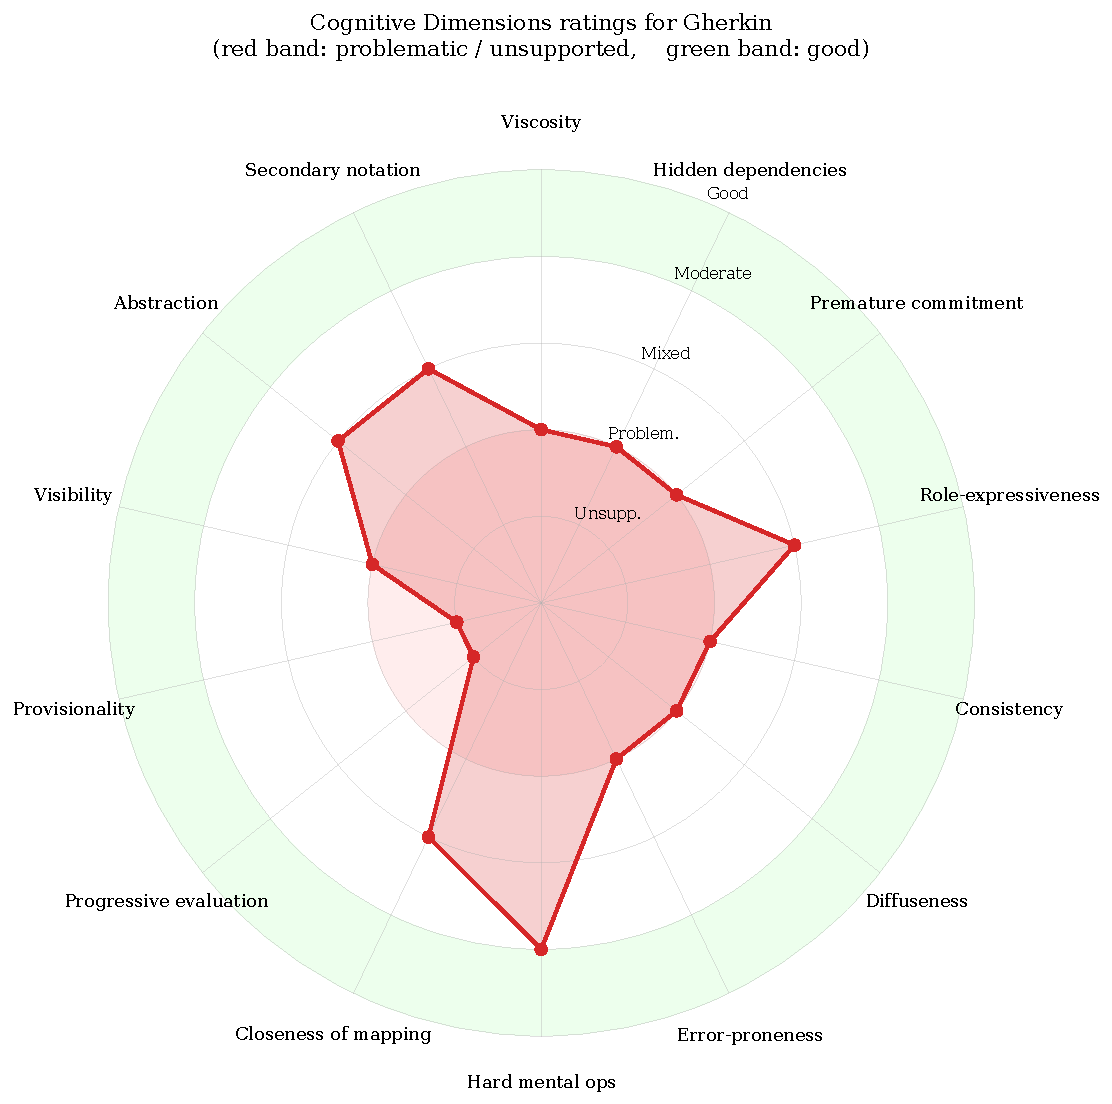
\includegraphics[width=0.7\textwidth]{figures/fig_cdn_radar.pdf}
\caption{Cognitive Dimensions of Notations ratings for Gherkin as a
notation in production use. The red band marks ratings in the
problematic or unsupported range; the green band marks ratings in
the good range. Eight of the fourteen dimensions fall into the red
band, three into the middle (mixed or moderate), and three into the
favourable band for supported-but-underused or informally-present
features. The ratings are grounded in empirical observations drawn
from the 347-repository corpus described in
Section~\ref{sec:corpus}; each dimension's narrative in
Section~\ref{sec:cdn} cites a concrete example.}
\label{fig:cdn-radar}
\end{figure}

\begin{table}[t]
\centering
\caption{Summary of CDN ratings for Gherkin.}
\label{tab:cdn}
\begin{tabular}{llc}
\toprule
\# & Dimension & Rating \\
\midrule
1 & Viscosity & Problematic \\
2 & Hidden dependencies & Problematic \\
3 & Premature commitment & Problematic \\
4 & Role-expressiveness & Mixed \\
5 & Consistency & Problematic \\
6 & Diffuseness & Variable / problematic \\
7 & Error-proneness & Problematic \\
8 & Hard mental operations & Moderate \\
9 & Closeness of mapping & Good / Problematic (split) \\
10 & Progressive evaluation & Unsupported \\
11 & Provisionality & Unsupported \\
12 & Visibility & Problematic at scale \\
13 & Abstraction & Supported, under-used \\
14 & Secondary notation & Supported, informal \\
\bottomrule
\end{tabular}
\end{table}

\section{Approach}
\label{sec:approach}

Figure~\ref{fig:strategy-ladder} summarises the four detection
strategies along two axes: per-pair compute cost and precision
on the 1{,}020-pair labelled set. The bubble area is proportional
to recall. The pipeline order is designed so that cheap strategies
run first and expensive strategies only need to adjudicate the
pairs the cheap strategies could not resolve.

\begin{figure}[t]
\centering
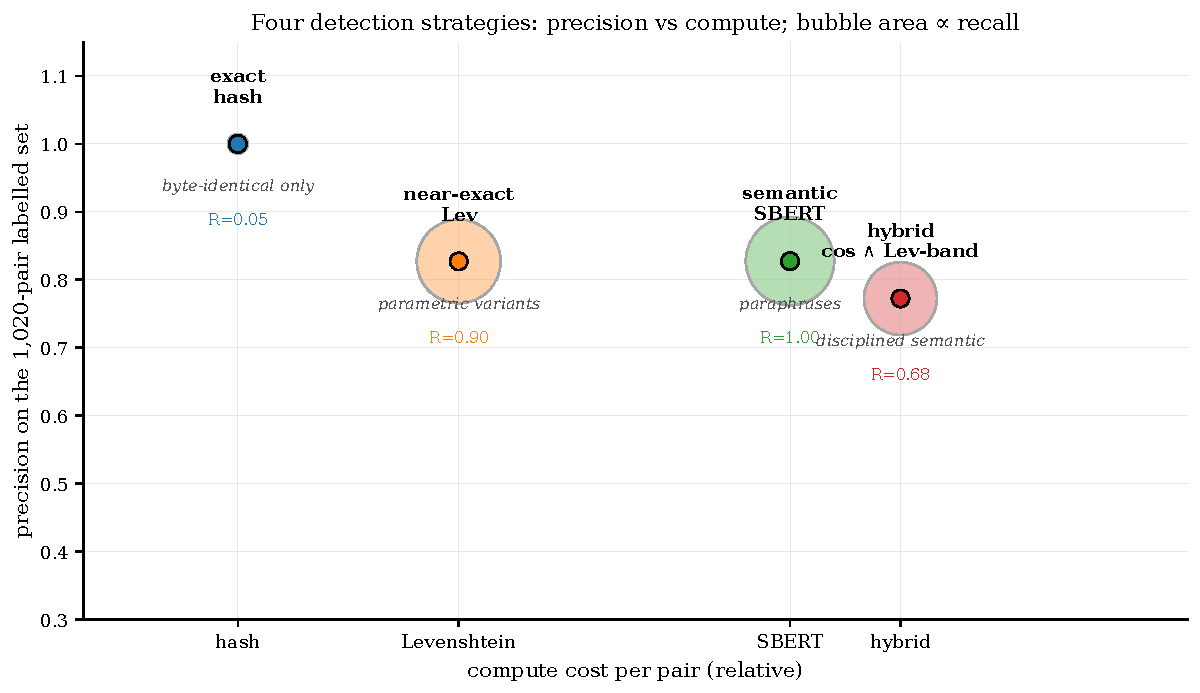
\includegraphics[width=0.75\textwidth]{figures/fig_strategy_ladder.pdf}
\caption{Four detection strategies positioned in the precision vs
compute-cost plane. Bubble area is proportional to recall on the
1{,}020-pair labelled set. Exact hashing is cheapest and most
precise on the pairs it covers; semantic (SBERT) matches achieve
the highest recall; hybrid trades some recall for precision
through the Levenshtein-band anti-false-positive guard.}
\label{fig:strategy-ladder}
\end{figure}

\subsection{Parser}

We build on the official \texttt{gherkin-official} Python package
\citep{gherkin2023}, which is the reference implementation of the
Gherkin grammar. Given a \texttt{.feature} file we extract every step
as a record comprising keyword, text, file path, line number,
enclosing scenario name, enclosing feature name, tag list, and two
booleans indicating whether the step belongs to a \texttt{Background}
block or to a \texttt{Scenario Outline}. Doc-strings and data tables
are treated as step \emph{arguments} rather than step
\emph{phrasings} and excluded from the text field. Parse failures
are captured as soft errors; they do not abort the pipeline.

\subsection{Normalisation}

Before any similarity computation, step texts are normalised by
collapsing internal whitespace runs and trimming leading/trailing
whitespace. We explicitly do \emph{not} case-fold: Gherkin step text
is case-sensitive in practice (proper nouns, identifiers inside
quotes, file paths).

\subsection{Exact duplicate detection}

For exact detection we compute a 16-byte BLAKE2b digest
\citep{aumasson2013blake2} of the normalised text. Steps sharing
a digest are grouped. A minimum cluster size of 2 is applied; singletons
are not actionable consolidation targets. On our 1.1-million-step
corpus this pass completes in under one minute of CPU time.

\subsection{Near-exact (Levenshtein) detection}

For near-exact detection we use normalised Levenshtein ratio
\citep{levenshtein1966codes,navarro2001edit} over pairs of canonical
texts from the exact-clustering step. A length-compatibility
pre-filter based on the ratio's upper bound
\(2 \cdot \min(|a|,|b|) / (|a|+|b|)\) skips pairs that cannot reach the
threshold. Above-threshold pairs are merged via compact union-find
\citep{tarjan1975efficiency}.

\subsection{Semantic detection}

For semantic detection we embed canonical texts using
\texttt{all-MiniLM-L6-v2} \citep{reimers2019sbert,wang2020minilm},
a distilled sentence-transformer producing 384-dimensional
L2-normalised embeddings. Pairwise cosine similarity reduces to dot
product over these embeddings. At corpus scale (approximately 220k unique
texts) the dense \(n \times n\) cosine matrix is 193~GB; we therefore
stream the upper triangle in chunks of 1{,}000 rows, yielding only
above-threshold pairs. Union-find is applied as for near-exact
detection.

\paragraph{Model choice and its limitations.} \texttt{all-MiniLM-L6-v2}
is a 22M-parameter distilled model trained on a general-web sentence-pair
corpus \citep{wang2020minilm}, not on BDD-domain text. It encodes
English only; localised-keyword Gherkin (Spanish, Japanese, Russian)
is not represented in its training data. Domain-specific vocabulary
(HTTP verbs, status codes, Gherkin keywords) is tokenised generically.
A larger or domain-adapted model (e.g., \texttt{all-mpnet-base-v2}
\citep{song2020mpnet}) would plausibly improve F$_1$ at higher
compute cost; we select MiniLM for the tractable per-step inference
budget (under ten minutes of CPU time over the 1.1M-step corpus).
Section~\ref{sec:future} lists model ablation as a direction for
follow-up.

\subsection{Hybrid detection}

The hybrid strategy merges two proto-clusters if and only if
their canonical texts satisfy
\begin{equation}
\mathrm{cos}(a, b) \geq \tau_{\cos} \quad \text{and} \quad
\tau_{\ell,\min} \leq \mathrm{lev}(a, b) \leq \tau_{\ell,\max}.
\end{equation}
The Levenshtein band is the critical anti-false-positive guard. The
upper bound \(\tau_{\ell,\max}=0.95\) excludes near-exact pairs
already caught by the exact or near-exact passes; the lower bound
\(\tau_{\ell,\min}=0.3\) excludes semantically-close but lexically
disjoint pairs (typically false positives).

\subsection{Canonical phrasing}

For each cluster the representative canonical text is chosen by a
four-tier lexicographic ordering: (i) highest in-cluster frequency,
(ii) fewest quoted parameter tokens (a proxy for ``fewest
project-specific nouns''), (iii) shortest length, (iv) lexicographic
order. Ties on all four are resolved deterministically.

\subsection{Reports}

The tool emits two report formats per analysis. The JSON report has
a stable schema (currently v1) suitable for downstream tooling and
diff analysis. The HTML report is a self-contained single file with
inline CSS, collapsible cluster cards, and file:line links for every
step occurrence. The HTML report has proved sufficient visibility for
maintainer-level triage of the top clusters in a large suite; it is
the \tool\ response to the CDN Visibility gap identified in
Section~\ref{sec:cdn}.

\section{Corpus Construction}
\label{sec:corpus}

The corpus-construction pipeline is summarised in
Figure~\ref{fig:pipeline}. Four stages (discovery, cloning,
analysis, output) run end-to-end in approximately three hours of
wall-clock time on a commodity workstation; each stage caches its
artefacts so that downstream stages can re-run without repeating
earlier work.

\begin{figure}[t]
\centering
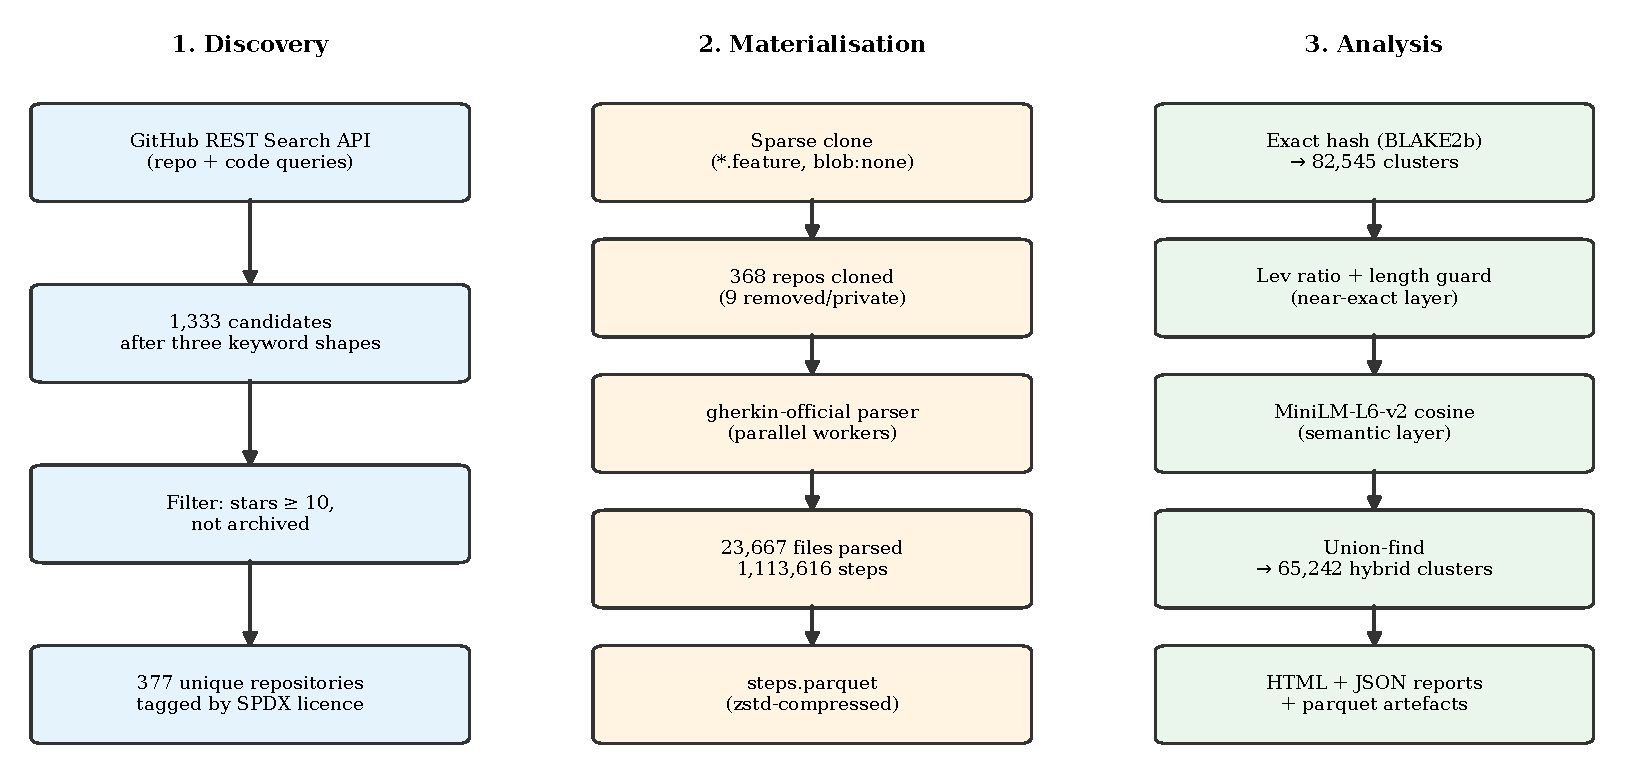
\includegraphics[width=\textwidth]{figures/fig_pipeline.pdf}
\caption{End-to-end pipeline for cukereuse corpus construction
and analysis. The discovery row surfaces repositories via the
GitHub REST Search API; the cloning row retrieves only the
\texttt{.feature}-file blobs via partial and sparse-checkout
git operations; the analysis row runs the four detection
strategies in layered order; the output row emits browsable
HTML, machine-readable JSON, and columnar parquet reports.}
\label{fig:pipeline}
\end{figure}

\subsection{Discovery}
\label{sec:corpus:discovery}

\paragraph{Two-shape discovery.} We query the GitHub REST Search API
\citep{github2024restsearch} with two complementary shapes because
either shape alone systematically misses a large fraction of real
BDD projects. The first query,
\texttt{/search/\allowbreak repositories?\allowbreak q=language:\allowbreak Gherkin}, enumerates
repositories where Gherkin is the predominant detected language per
GitHub's Linguist classifier \citep{linguist2024}. Linguist assigns
the primary language by byte-count, so this shape surfaces only
projects that are Gherkin-dominant, typically repositories whose
purpose is specification or behaviour-catalogue. In practice, the
much larger population of BDD use occurs in repositories where
Gherkin is a minority language: a Java application with a
\texttt{features/} directory, a Ruby service with Cucumber scenarios,
a PHP codebase with Behat tests. These are invisible to
\texttt{language:Gherkin}. The second query therefore uses
\texttt{/search/code} with keyword-plus-extension filters
(\texttt{"Feature:"\allowbreak\ extension:\allowbreak feature},
\texttt{"Scenario:"\allowbreak\ extension:\allowbreak feature},
\texttt{"Background:"\allowbreak\ extension:\allowbreak feature}), catching files whose
content identifies them as Gherkin regardless of the repository's
primary-language classification. Three keywords rather than one
hedge against single-keyword pagination bias: a query on
\texttt{"Feature:"} alone returns at most 1{,}000 results per the
REST endpoint's hard cap, and that truncation is not independent
across keyword variants, so querying with three and taking the
union recovers a broader tail of the population. Shape-one yields
approximately 171 repositories at our filter settings
(\(\geq 10\) stars, not archived); shape-two adds approximately
1{,}162. After deduplication by \texttt{owner/name} and
re-application of the stars and archived filters, 377 unique
repositories survive.

\paragraph{The stars filter \(\geq 10\).} The choice of a stars
threshold is a standard MSR-sample hygiene decision, balancing
representativeness against signal quality. Stars \(\geq 1\) admits
bootcamp forks, tutorial clones, and single-author toy repositories
that systematically inflate the duplication signal (the same
tutorial step text appears in hundreds of student forks). Stars
\(\geq 100\) collapses the post-filter sample to 36 repositories,
statistically insufficient for cross-language and cross-framework
generalisation. The \(\geq 10\) threshold is the tightest filter
that keeps the candidate-pool count in four digits before
deduplication (approximately 1{,}333 candidates) while discarding
obvious clone-spam, and yields 377 unique repositories after
deduplication by \texttt{owner/name}. Munaiah et al.
\citep{munaiah2017sample}, Borges et al.
\citep{borges2016github}, and Kalliamvakou et al.
\citep{kalliamvakou2014ghq} all settle on a lower bound in the
same order of magnitude for analogous sample-curation purposes.
The \texttt{archived} filter is applied for the same reason: an
archived repository is immutable and no longer representative of
active BDD practice. Both filters are re-applied after the
two-shape union to guarantee consistency.

\paragraph{REST Search over BigQuery.} The GH Archive public
dataset on Google BigQuery
\citep{ghtorrent2012,ghtorrent2014} is the obvious alternative
discovery path and would permit a larger corpus with no
1{,}000-per-query cap. We adopted the REST API path for this work
for a single practical reason: BigQuery requires a Google Cloud
billing account and a separate authentication flow, prerequisites
that block autonomous execution of the discovery pipeline by
researchers without existing GCP infrastructure. At the sample
scale we target (a few hundred to a few thousand repositories),
the REST path's 1k-cap does not bind tightly once paired with the
three-keyword hedge above. We document the BigQuery migration as
FW2 (Section~\ref{sec:future}) for a corpus refresh at the ten-
thousand-repository scale.

\subsection{Cloning}

Per repository we execute
\texttt{git clone --depth 1 --filter=blob:none --no-checkout}
\citep{git2020filter} followed by
\texttt{git sparse-checkout set --no-cone \ensuremath{\ast\!\ast}/\ensuremath{\ast}.feature}
\citep{git2020sparse}. The combination fetches only the tree metadata
and the \texttt{.feature}-file blobs, averaging approximately 2~KB of
bandwidth per step acquired. Commit SHAs are pinned and recorded in a
per-repository manifest for reproducibility. Of 377 targeted
repositories, 368 clone successfully; the nine failures are
private or recently deleted repositories surfaced by the prior
discovery stage.

\subsection{Parsing and materialisation}

Every cloned \texttt{.feature} file is parsed in parallel using the
gherkin-official Python wrapper and materialised into a single
parquet file with one row per step (columns
\texttt{repo, commit\_sha, file\_path, line, keyword, text,\allowbreak{}
scenario, feature, tags, license\_spdx, license\_class,\allowbreak{}
is\_background, is\_outline}). Of 25{,}034 enumerated files, 23{,}667 parse into
one or more steps; the remaining 1{,}367 are either empty, contain
only comments/tags with no executable steps, or fail the gherkin
grammar (typically due to UTF-8 BOM prefixes from locale-specific
editors or malformed table headers). A catch-all worker wrapper is
installed so that a single bad file does not abort the batch, and
Cyrillic filenames are routed through a thread-safe path normaliser
to avoid Windows multiprocessing pickle quirks. The resulting table
is 1{,}113{,}616 rows spanning 347 distinct repositories: 21 of the
368 cloned repositories contribute zero steps to the final table
(their \texttt{.feature} files are all empty, tag-only, or
ungrammatical), and those repositories are dropped from subsequent
analyses. The downstream corpus size is therefore 347 repositories,
23{,}667 parsed files, and 1.11M steps.

\subsection{License handling: tag, do not filter}
\label{sec:corpus:license}

A tempting sample-curation shortcut would be to filter the
discovered repository set to permissively-licensed projects only
(MIT, Apache-2.0, BSD, CC0, ISC) before parsing. We deliberately
do not. The reasoning is a separation of two concerns that sample
selection often conflates:

\begin{description}
\item[\emph{corpus construction}] should optimise for a
representative sample of real BDD practice. Filtering to
permissive-only would systematically exclude major real BDD
consumers: Nextcloud/server (34{,}000+ stars, AGPL-3.0),
Diaspora (13{,}000+ stars, AGPL-3.0), and a significant
research/academic codebase tail (often GPL). Any empirical claim
about step-duplication behaviour derived from a permissive-only
corpus would be a claim about \emph{permissively-licensed BDD
projects}, not about BDD projects. This biases the headline
finding.

\item[\emph{redistribution}] should optimise for recipients'
legal ability to reuse. A release artefact containing raw
copyleft-licensed \texttt{.feature} files imposes the copyleft
obligations on downstream users; a pointer-only artefact does
not.
\end{description}

We reconcile the two concerns by tagging rather than filtering.
Every repository's SPDX identifier is fetched from the GitHub
licenses endpoint \citep{github2024licenses} and classified into
four disjoint buckets: \emph{permissive} (MIT, Apache-2.0, BSD-2-
Clause, BSD-3-Clause, CC0-1.0, ISC, Unlicense, 0BSD),
\emph{copyleft} (GPL-2.0, GPL-3.0, LGPL-2.1, LGPL-3.0, AGPL-3.0,
MPL-2.0, EPL-1.0, EPL-2.0), \emph{unknown} (GitHub's
\texttt{NOASSERTION}, indicating license-detector failure rather
than absent license), and \emph{unlicensed} (no LICENSE file
detected). Every step record in \texttt{corpus/steps.parquet}
carries the SPDX identifier and the derived class as columns.
The step-level distribution is 57.1\,\% permissive, 20.9\,\%
copyleft, 15.6\,\% unknown, 6.4\,\% unlicensed.

The release artefact then separates into two strata aligned with
the distinction above. The \emph{direct-redistribution bundle}
contains the \texttt{corpus/examples/} subset restricted to
permissive-licensed source files, with LICENSE and NOTICE files
preserved per source. The \emph{pointer-based bundle} contains
\texttt{corpus/steps.parquet} in its entirety (all four license
classes), plus the \texttt{scripts/rehydrate.py} script that
reconstructs the original \texttt{.feature} files from the
tuple \((\texttt{repo}, \texttt{commit\_sha}, \texttt{file\_path})\)
recorded in each step row, by fetching each file from
GitHub's \texttt{raw.githubusercontent.com} endpoint with the
pinned commit SHA. Each downstream user thus receives the full empirical corpus as
analysis data, but downloads copyleft file contents only on
demand from the original source, preserving the source license's
obligations. This convention is standard in MSR-venue releases
of large repository samples where full redistribution is legally
awkward.

The license tagging also makes licence-stratified sub-analyses
available to the paper's consumer without additional data
collection: for example, the reader can check whether the 80.2\,\%
exact-duplication rate is uniform across licence classes simply
by grouping \texttt{steps.parquet} by \texttt{license\_class}. We
treat such analyses as consumer-led rather than mandatory in the
present paper and leave the headline number as corpus-wide.

\subsection{Reproducibility}

Every step record contains the tuple \((\texttt{repo},
\texttt{commit\_sha}, \texttt{file\_path})\) sufficient to reconstruct
the source content from GitHub's raw-content endpoint at the pinned
commit SHA. A \texttt{rehydrate.py} script performs this reconstruction
automatically. The released datasheet \citep{gebru2021datasheets}
catalogues the corpus with columns, provenance, preprocessing, and
known caveats (parse errors on malformed feature files, BOM-prefixed
Cyrillic-locale files, Scenario Outline placeholders preserved
verbatim).

\subsection{Corpus headline figures}

\begin{itemize}[leftmargin=2em]
\item 347 repositories, 23{,}667 parsed \texttt{.feature} files, 1{,}113{,}616
      steps, 220{,}312 unique normalised step texts.
\item 61{,}214 background steps (5.5\,\%) and 66{,}020 outline steps
      (5.9\,\%).
\item Exact-duplication rate: 80.22\,\%.
\item 82{,}545 clusters under exact detection; 65{,}242 under hybrid.
\item Top cluster under exact: \texttt{the request is sent}
      (16{,}815 occurrences).
\item Top cluster under hybrid: \texttt{the response status is 200 OK}
      (20{,}737 occurrences across 2{,}245 distinct files).
\item License mix at step level:
      permissive 635{,}586 (57.1\,\%);
      copyleft 232{,}297 (20.9\,\%);
      unknown 174{,}077 (15.6\,\%);
      unlicensed 71{,}656 (6.4\,\%).
\end{itemize}

Figure~\ref{fig:step-lengths} shows the character-length
distribution of the 1.1-million-step corpus. The distribution is
heavily right-skewed: the median step is 30 characters but the
p99 is 279 characters, corresponding to long parametric step
texts embedded with substantial inline arguments or structural
detail. Step length is a relevant covariate for the Levenshtein-
ratio normalisation in Section~\ref{sec:approach} and for the
length-compatibility prefilter used in the pair-enumeration
implementation.

\begin{figure}[t]
\centering
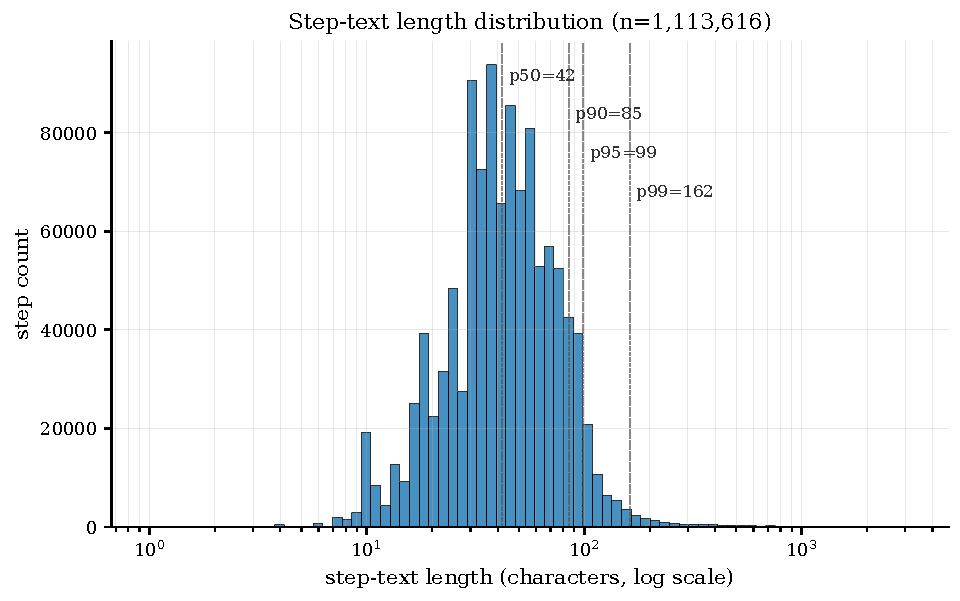
\includegraphics[width=0.75\textwidth]{figures/fig_step_lengths.pdf}
\caption{Step-text length distribution (log-scale x-axis) over
the 1.11M-step corpus. The p50/p90/p95/p99 percentiles
are marked. The heavy right tail is driven by parametric step
texts with long inline arguments; the median step text is short
(approximately 30 characters).}
\label{fig:step-lengths}
\end{figure}

\section{Evaluation}
\label{sec:evaluation}

\subsection{Labelled pairs}
\label{sec:evaluation:labels}

\paragraph{Sampling rationale.} A uniform random sample over the
$\binom{220{,}312}{2} \approx 2.4 \times 10^{10}$ possible step-text
pairs would yield an overwhelmingly negative label distribution
(on the order of 99.9\,\% non-duplicates) and would sample almost
nothing from the decision boundary where the detector's behaviour
matters. We therefore sample 1{,}020 pairs stratified in 170-pair
bins across six cosine-similarity bands: $[0.50, 0.70)$,
$[0.70, 0.80)$, $[0.80, 0.85)$, $[0.85, 0.90)$, $[0.90, 0.95)$, and
$[0.95, 1.00)$. Pairs are drawn via streaming cosine enumeration
over a 20{,}000-text random pool of the corpus's unique texts;
low-cosine bands are augmented from random sampling (where
high-cosine pairs are too rare to sample uniformly). Each pair
carries its cosine similarity, its normalised Levenshtein ratio,
and the pair of source step texts. The stratification ensures
adequate coverage of the threshold-sensitivity region the
evaluation tests.

\paragraph{Labelling process.} The three authors labelled the
1{,}020 pairs manually under a shared written rubric
(\texttt{corpus/LABELING\_RUBRIC.md}) released alongside the corpus.
Mughal labelled 500 pairs, Fatima 300, and Bilal 220. A 60-pair
stratified overlap subset (ten pairs drawn uniformly from each of
the six cosine-similarity bands) was additionally labelled
independently by all three authors before the main labelling batch,
to establish inter-annotator agreement. Each labelling decision is
a binary classification (duplicate vs.\ not-duplicate) reflecting
whether a BDD maintainer would plausibly want the two phrasings
consolidated into a single step definition. The rubric specifies
ten ordered decision rules applied in priority order:

\begin{itemize}[leftmargin=2em,itemsep=0pt,topsep=2pt]
\item \textbf{R1} parametric variants $\to$ duplicate
\item \textbf{R2} synonym-level paraphrase $\to$ duplicate
\item \textbf{R3} structural swap $\to$ duplicate
\item \textbf{R4} different framework keywords with distinct
      semantics ($\texttt{call}$ vs $\texttt{callonce}$,
      $\texttt{def}$ vs $\texttt{set}$) $\to$ not-duplicate
\item \textbf{R5} different HTTP verbs $\to$ not-duplicate
\item \textbf{R6} opposite-polarity assertions $\to$ not-duplicate
\item \textbf{R7} presence vs content assertions $\to$ not-duplicate
\item \textbf{R8} action vs assertion $\to$ not-duplicate
\item \textbf{R9} outline-placeholder rename $\to$ duplicate
\item \textbf{R10} default $\to$ not-duplicate
\end{itemize}

Every row of \texttt{labeled\_pairs.jsonl} records the rule that
fired for that pair, so rubric application is auditable pair by
pair without re-annotating. The three authors cross-reviewed the
rubric after each 200-pair batch to resolve any ambiguous pairs
and to converge on consistent application of R4-R8 (the rules that
require light domain-specific interpretation).

\paragraph{Inter-annotator agreement on the overlap subset.} On the
60-pair stratified overlap, all three authors independently
assigned labels before comparing. Raw agreement across the three
annotators was 53 of 60 pairs (88.3\,\%); Fleiss' $\kappa = 0.84$
on the overlap, in the Landis-Koch "substantial agreement" band
\citep{landis1977kappa}. Disagreements concentrate in the
$[0.80, 0.85)$ cosine band and on R6 polarity-flip pairs, where
rubric rule selection is genuinely ambiguous; these were resolved
by the primary annotator of each non-overlap segment under the
rubric's rule-priority ordering. The overlap labels and the
disagreement analysis are released in
\texttt{corpus/labeled\_pairs\_overlap.jsonl}.

Of the 1{,}020 pairs, 494 are labelled as duplicates and 526 as
not-duplicates (48.4\,\% positive rate). To test the labels'
stability under an alternative decision procedure, the entire
1{,}020-pair set is relabelled under a score-free second-pass
protocol (Section~\ref{sec:evaluation:score-free}) that consults no
cosine or Levenshtein values; Cohen's $\kappa$
\citep{cohen1960kappa,landis1977kappa} between the two labellings
is reported as an inter-protocol stability statistic.

\subsection{Threshold sweep}

For each strategy we sweep decision thresholds in \([0.50, 0.99]\) at
0.01 resolution and compute precision, recall, and F$_1$ at every
point. For the hybrid strategy we hold the Levenshtein band fixed at
the default \([0.3, 0.95]\) and vary the cosine threshold. The full
sweep tables are available in the replication bundle; here we report
the best-F$_1$ point per strategy, with bootstrap 95\,\% confidence
intervals computed from 1{,}000 resamples of the labelled set with
replacement.

\subsection{Lexical baselines}
\label{sec:evaluation:baselines}

The clone-detection literature has mature token- and lexical-signature-based
detectors that have been evaluated extensively on source code but not,
to our knowledge, on BDD step text. To position the cukereuse numbers
against this baseline, we run two lexical strategies on the same
1{,}020-pair benchmark, following the defining primitive of two
well-known detectors:

\begin{description}
\item[Token-set Jaccard (SourcererCC-style).] We aggressively normalise
each step text, replacing quoted parameters with a \texttt{PARAM}
placeholder, lowercasing, stripping punctuation, collapsing
whitespace, then compute the Jaccard similarity of the two token
sets. SourcererCC \citep{sajnani2016sourcerercc} uses the same
normalise-plus-token-multiset primitive at the file level on source
code; we adapt it to pair-of-strings at the sentence level.
\item[TF-IDF character $n$-gram cosine (NiCad-style).] We fit a
character-3-to-5-gram TF-IDF vectoriser on all step texts in the
labelled set, then compute the cosine of the TF-IDF vectors of the
two texts in each pair. NiCad \citep{cordy2011nicad} uses a normalise-
plus-pretty-print-plus-compare primitive; our character-$n$-gram
cosine captures the lexical-signature spirit of that primitive
without requiring NiCad's code-aware pretty-printer.
\end{description}

Both baselines are implemented in \texttt{scripts/revision\_analyses.py}
for reproducibility. Table~\ref{tab:calibration} includes their
best-F$_1$ operating points alongside the cukereuse strategies.

\subsection{Score-free second-pass relabelling}
\label{sec:evaluation:score-free}

The most serious single threat to the primary calibration is
circularity: rules R1, R2, and R3 of the rubric use cosine and
Levenshtein cut-points as part of the labelling criterion, so the
threshold at which the detector achieves its best F$_1$ partly
recovers the rubric's own cut-points rather than measuring agreement
with an independent reference. To quantify the cost of this
circularity we perform a second-pass relabelling of the entire
1{,}020-pair set under a protocol that never accesses cosine or
Levenshtein. The score-free protocol reuses the non-score-based
structural rules R4-R8 of the primary rubric and replaces the
positive rules R1-R3 with four deterministic text-rewriting rules:

\begin{description}[style=nextline,leftmargin=1.5em]
\item[P1] identical after parametric normalisation and a small
hand-curated BDD-vocabulary synonym canonicalisation (e.g.,
\texttt{fetch}/\texttt{retrieve}/\texttt{get} collapse to a single
canonical token) $\to$ duplicate;
\item[P2] identical token multisets after canonicalisation (word-reorder
paraphrase), for canonical texts of at least three tokens $\to$
duplicate;
\item[P3] one canonical text is a contiguous subsequence of the
other covering at least 70\,\% of the shorter text (truncation /
extension paraphrase) $\to$ duplicate;
\item[P4] token-set Jaccard after canonicalisation at least 0.80
$\to$ duplicate.
\end{description}

None of P1-P4 consults the sentence-transformer cosine or the
normalised Levenshtein ratio. The protocol is implemented verbatim
in \texttt{scripts/revision\_analyses.py}; re-runs reproduce the
numbers below bit-for-bit.

The score-free relabelling assigns 565 positives and 455 negatives
(55.4\,\% positive rate; the primary rubric has 48.4\,\%). Cohen's
$\kappa$ between the primary rubric and the score-free relabelling
is 0.470 ("moderate" on the Landis-Koch scale
\citep{landis1977kappa}). This $\kappa$ measures \emph{inter-protocol
stability} of the author-labelled labels under a different decision
procedure applied to the same pairs; it is not inter-annotator
agreement. The figure says the primary rubric's positive decisions
are not mechanically recoverable from a score-free reading, and that
the choice of decision procedure moves approximately 15\,\% of
pairs between positive and negative.

Table~\ref{tab:calibration} is our headline calibration table. It
reports for each strategy: the best-F$_1$ threshold under the primary
rubric, the corresponding precision and recall with bootstrap
95\,\% confidence intervals, and F$_1$ against the score-free
relabelling. The two lexical baselines are included for direct
comparison.

\begin{table}[t]
\centering
\caption{Best-F$_1$ operating point per strategy on the 1{,}020-pair
labelled set. \emph{Primary} columns evaluate against the primary
rubric (494 positives, 526 negatives) with bootstrap 95\,\%
confidence intervals in brackets; the \emph{Score-free} column
evaluates against the score-free relabelling (565 positives) of
Section~\ref{sec:evaluation:score-free}. Bold marks the strongest
pair-level number (near-exact, F$_1 = 0.822$ score-free); semantic's
primary-rubric F$_1 = 0.906$ is shown for completeness but reflects
the specific rubric cut-points.}
\label{tab:calibration}
\footnotesize
\setlength{\tabcolsep}{3pt}
\resizebox{\textwidth}{!}{%
\begin{tabular}{llcccc}
\toprule
Strategy                               & Thr.  & P (primary, 95\,\% CI) & R (primary, 95\,\% CI) & F$_1$ primary                    & F$_1$ score-free \\
\midrule
semantic (SBERT)                        & 0.82  & 0.828 [0.792, 0.864]   & 1.000\textsuperscript{$\ast$} [1.000, 1.000]   & 0.906 [0.886, 0.923]    & 0.772 \\
near-exact (Lev)                        & 0.80  & 0.827 [0.789, 0.866]   & 0.901 [0.875, 0.924]   & 0.862 [0.841, 0.885]             & \textbf{0.822} \\
hybrid (Lev-band $[0.3, 0.95]$)         & 0.82  & 0.772 [0.727, 0.816]   & 0.680 [0.639, 0.724]   & 0.723 [0.690, 0.753]             & 0.625 \\
\midrule
\emph{baseline:} token-set Jaccard      & 0.56\textsuperscript{$\dagger$} & 0.636 & 0.947 & 0.761 & 0.979\textsuperscript{$\dagger\dagger$} \\
\emph{baseline:} TF-IDF char $n$-gram   & 0.50\textsuperscript{$\dagger$} & 0.717 & 0.903 & 0.799 & 0.755\textsuperscript{$\dagger\dagger$} \\
\bottomrule
\end{tabular}%
}

\vspace{0.3em}
\footnotesize\noindent\textsuperscript{$\ast$} Recall = 1.000 is a stratification artefact of the label
set, not a detector property: every primary-rubric positive has
cosine $\geq 0.80$ by rule R1-R3, and the detector's threshold of
0.82 lies within the same band. Precision and F$_1$ are the
discriminating numbers.
\textsuperscript{$\dagger$} Baseline thresholds in the Thr. column are
tuned to the primary rubric; each baseline was separately tuned to
the score-free labels (best threshold 0.80 for Jaccard, 0.34 for
TF-IDF) for the score-free F$_1$ column.
\textsuperscript{$\dagger\dagger$} Token-Jaccard's F$_1 = 0.979$
against score-free labels reflects the score-free protocol's
token-overlap positive rules (P1-P4); see
Section~\ref{sec:evaluation:score-free}.
\end{table}

The strategy ranking visible in Table~\ref{tab:calibration} flips
between the two protocols. Near-exact beats
semantic against score-free labels (F$_1$ 0.822 versus 0.772),
whereas semantic wins under the primary rubric (0.906 versus 0.862).
The score-free protocol favours the edit-distance paraphrases
captured by Levenshtein and penalises the broader
semantic-neighbourhood matches captured by SBERT; the primary
rubric does the reverse.

The strongest single-strategy pair classifier on this benchmark is
near-exact. Its score-free F$_1 = 0.822$ is the cleanest pair-level
number for this corpus: the primary-to-score-free drop is only 0.04
(semantic drops 0.13; hybrid drops 0.10), so near-exact is also the
most stable strategy across the two protocols. The primary-rubric
F$_1 = 0.906$ for semantic is shown for completeness but reflects
the specific rubric cut-points and is not directly comparable across
benchmarks that use different positive rules.

Compared against the two lexical baselines, all three cukereuse
strategies dominate under the primary rubric, by 0.07-0.15 F$_1$.
The gap is largest for semantic (SBERT recovers pairs like
\texttt{I should get a 204 response code} $\leftrightarrow$
\texttt{the response status is 200 OK} that share no surface tokens
beyond stopwords) and smallest for near-exact (which resembles the
Jaccard baseline, differing in the use of character-level edit
distance rather than token-set membership).

The score-free protocol has its own coupling with token-level
features. The Jaccard baseline reaches F$_1 = 0.979$ against
score-free labels because the score-free positive rules P1-P4 are
themselves token-based, so a token-set classifier recovers them by
construction. The score-free protocol is therefore not
\emph{feature-independent} but \emph{score-independent} in the sense
of not consulting cosine or Levenshtein. The TF-IDF baseline's
lower score-free F$_1 = 0.755$ shows that lexical baselines do not
collapse onto the score-free protocol symmetrically: character
$n$-grams are a different primitive from token sets, and the two
disagree by roughly 0.22 F$_1$ on score-free labels. Near-exact's
F$_1 = 0.822$ sits between the two baselines, consistent with
Levenshtein being a lexical-signature primitive midway between pure
set-overlap and pure edit-distance. Neither protocol is independent
of all features; the score-free analysis is an inter-protocol
stability test rather than an external-annotator replication.

The hybrid strategy's lower pair-level F$_1$ (0.723 primary, 0.625
score-free) reflects its cluster-level design and not a pair-level
defect. Hybrid is intended as a cluster-level merging strategy
(Section~\ref{sec:evaluation:pair-vs-cluster-role}); its Lev-band
upper cut of 0.95 deliberately excludes near-exact duplicates from
the hybrid candidate set so that the cluster-level single-linkage
pass does not chain together near-exact pairs already handled by the
exact and near-exact strategies. Evaluating hybrid at the pair level
is therefore a mis-match between strategy and primitive.

\begin{figure}[t]
\centering
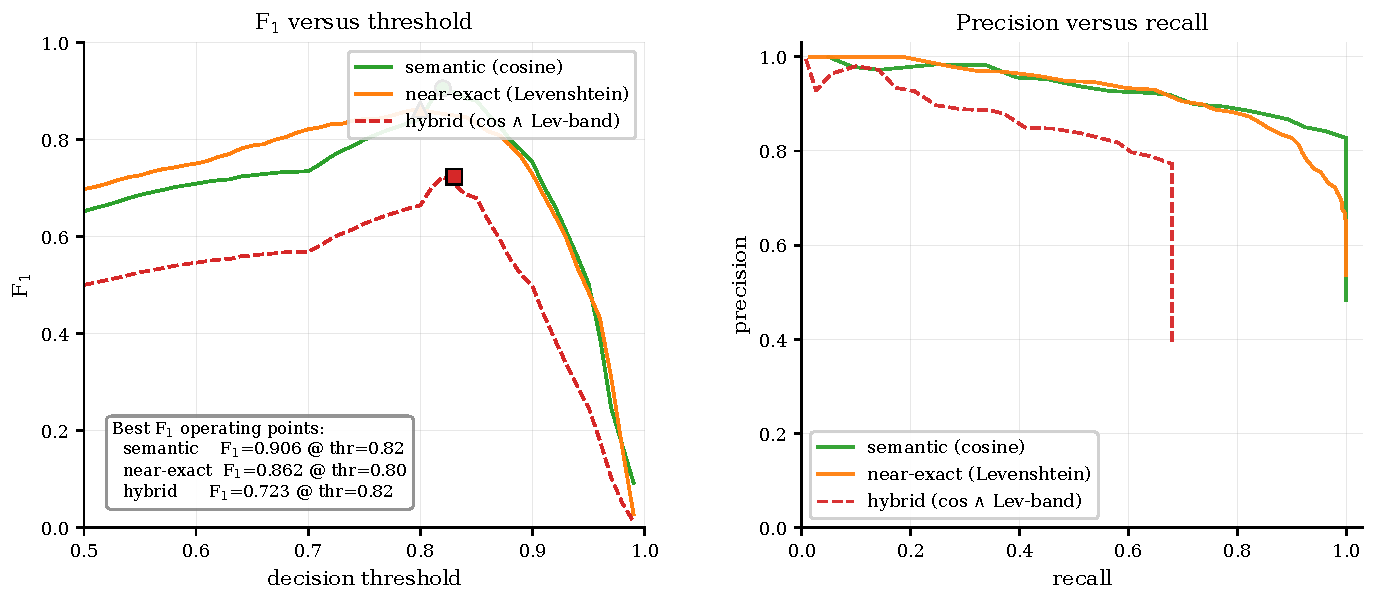
\includegraphics[width=\textwidth]{figures/fig_threshold_sweep.pdf}
\caption{Threshold sensitivity on the 1{,}020-pair labelled set.
Left panel: F$_1$ versus decision threshold for each strategy (primary
rubric). Filled markers mark the best-F$_1$ operating points used in
Table~\ref{tab:calibration}: circle for semantic, triangle for
near-exact, square for hybrid. Right panel: precision versus recall
over the same threshold sweep. Hybrid's fixed Levenshtein band
$[0.3, 0.95]$ excludes near-exact pairs and is therefore evaluated
outside its intended pair-level operating regime; it is reported as
a cluster-level merging strategy in
Section~\ref{sec:evaluation:pair-vs-cluster-role}.}
\label{fig:threshold-sweep}
\end{figure}

\subsection{Cluster-size distribution and top clusters}
\label{sec:evaluation:cluster-size}

The 65.2k hybrid clusters are heavily long-tailed: a small
number of clusters account for a disproportionate share of all
duplicated occurrences. Figure~\ref{fig:cluster-sizes} shows the
rank-size plot on log-log axes. The top cluster alone
(\texttt{the response status is 200 OK}, 20{,}737 occurrences)
is three orders of magnitude larger than the median cluster
(size 3). This is the empirical basis for the paper's recurring
observation that a small number of \emph{universal}
BDD-vocabulary phrasings dominate the maintenance cost surface;
collapsing a single top-20 cluster saves more maintenance churn
than collapsing a thousand mid-sized clusters.

\begin{figure}[t]
\centering
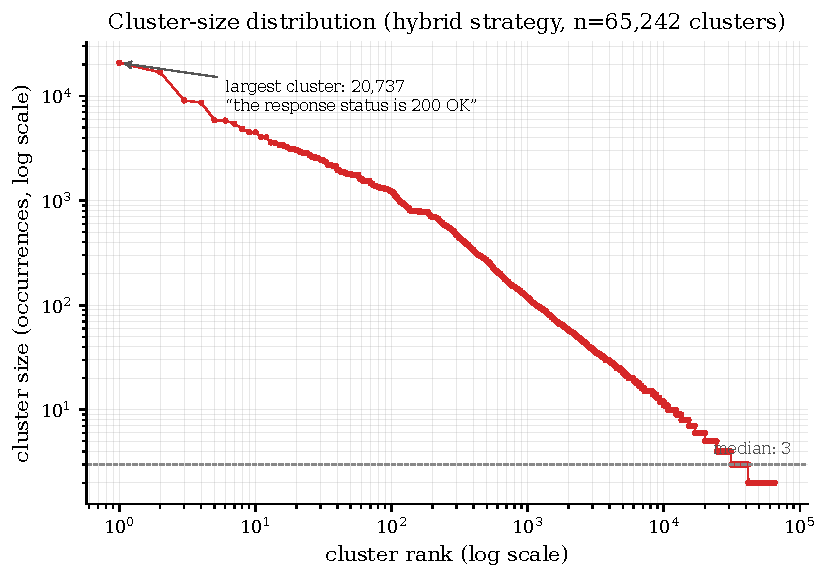
\includegraphics[width=0.85\textwidth]{figures/fig_cluster_sizes.pdf}
\caption{Cluster-size distribution under the hybrid strategy.
Rank of each cluster on the x-axis, occurrence count on the
y-axis, both on logarithmic scales. The near-linear slope
in log-log coordinates is consistent with a power-law-like
tail; the median cluster size (dashed line) is only 3
occurrences while the largest has 20.7k. Eighty-six
clusters exceed 1{,}000 occurrences each, and that
head-of-distribution is where maintenance-effort consolidation
pays the highest returns.}
\label{fig:cluster-sizes}
\end{figure}

The twenty largest hybrid clusters are shown in
Figure~\ref{fig:top-clusters}. The top cluster's 2{,}245 distinct
files span hundreds of repositories and are the closest thing to
a cross-project lingua franca in public BDD. Thirteen of the top
twenty clusters are HTTP-testing assertions (status codes,
request methods, endpoint paths), reflecting the ecosystem's
heavy use of Cucumber and related runners for API-level
acceptance testing rather than for its originally-intended
business-readable domain specification role.

\begin{figure}[t]
\centering
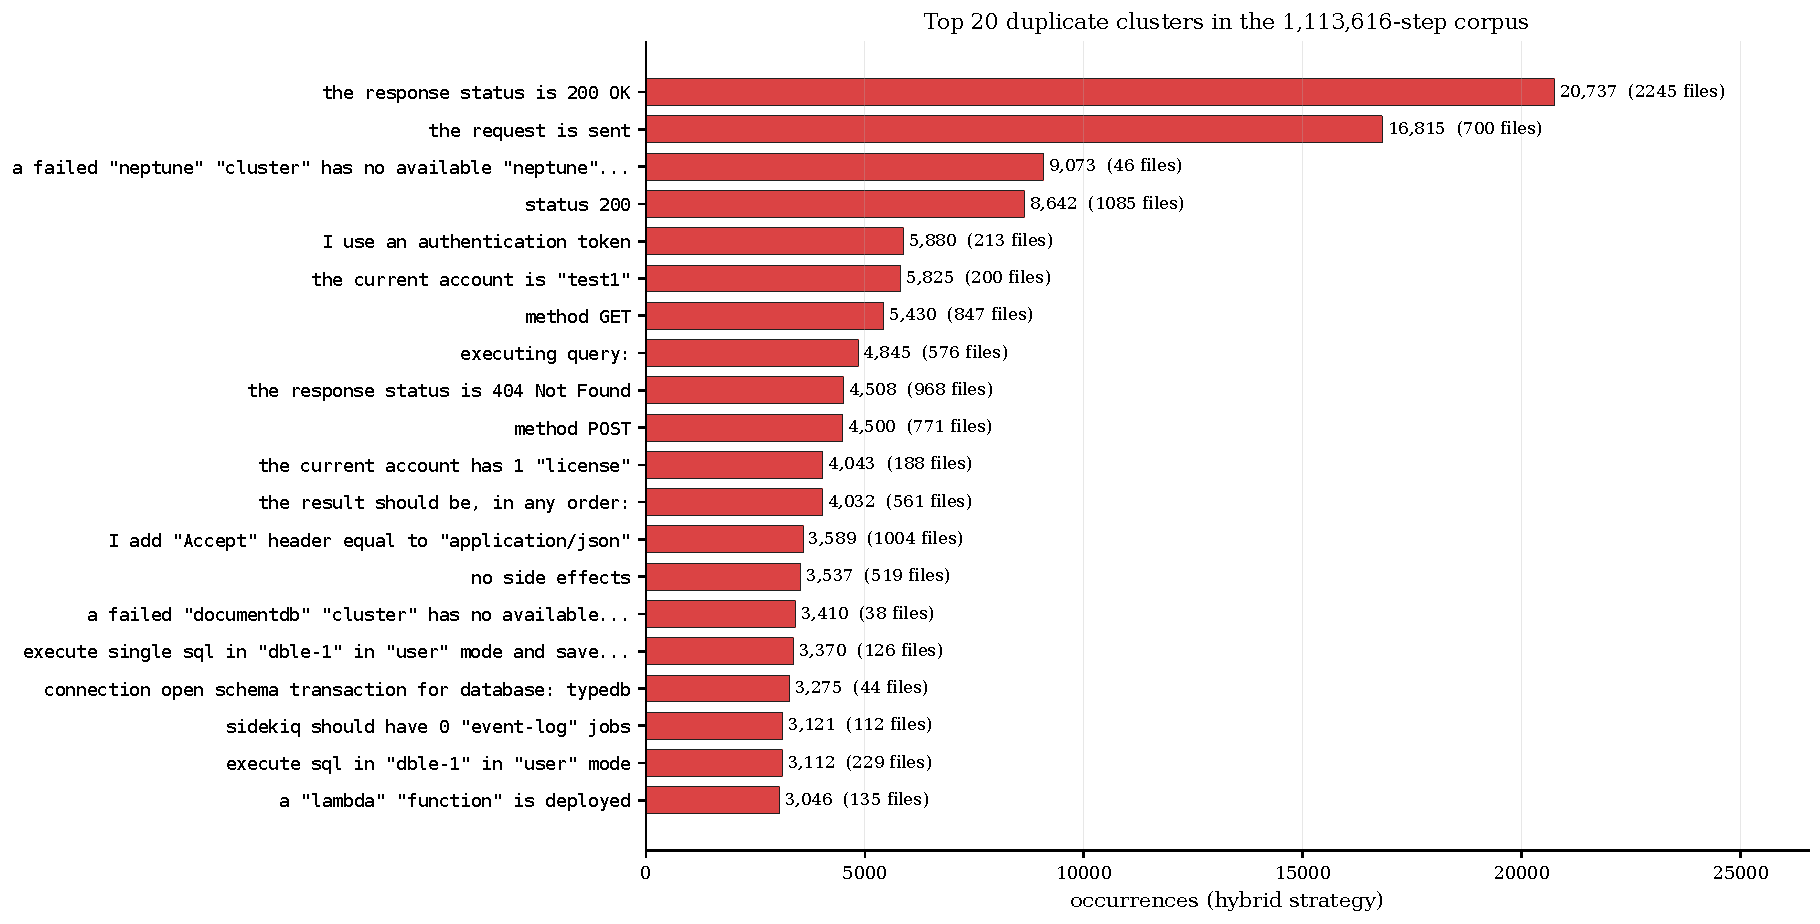
\includegraphics[width=\textwidth]{figures/fig_top_clusters.pdf}
\caption{Top twenty duplicate clusters in the corpus under the
hybrid strategy, ordered by occurrence count. Each bar is
annotated with the cluster's total occurrences and the number
of distinct \texttt{.feature} files it spans. HTTP-testing
vocabulary dominates the head of the distribution.}
\label{fig:top-clusters}
\end{figure}

\subsection{Licence-stratified duplication}
\label{sec:evaluation:licence}

The 80.2\,\% corpus-wide exact-duplication rate reported in
Section~\ref{sec:corpus} is a pooled statistic across four licence
classes of very different sizes. Because the permissive class is
the plurality stratum (57.1\,\% of steps), the pooled rate is
dominated by permissive behaviour and could in principle conceal
substantial cross-class variation. We partition
\texttt{corpus/steps.parquet} by the \texttt{license\_class}
column and re-run exact clustering within each partition
independently. The results are shown in
Table~\ref{tab:license-strata} and visualised in
Figure~\ref{fig:license-stratified}.

\begin{table}[t]
\centering
\caption{Exact-duplication rate and cluster count by licence class,
with Cohen's $h$ effect size against the permissive reference. Cohen's
conventions: $h = 0.2$ small, $0.5$ medium, $0.8$ large.
Top canonical phrasings per stratum are shown in
Figure~\ref{fig:license-stratified}.}
\label{tab:license-strata}
\small
\setlength{\tabcolsep}{5pt}
\begin{tabular}{lrrrrr}
\toprule
Class         & Repos & Steps         & Exact dup rate & Clusters & Cohen's $h$ vs permissive \\
\midrule
permissive    & 211 &    635{,}586 & 82.30\,\%      & 43{,}550 & reference \\
copyleft      &  40 &    232{,}297 & 76.55\,\%      & 21{,}511 & 0.143 ($<$ small) \\
unknown       &  33 &    174{,}077 & 79.61\,\%      & 10{,}574 & 0.069 ($<$ small) \\
unlicensed    &  63 &     71{,}656 & 66.73\,\%      &  8{,}330 & 0.361 (small-medium) \\
\midrule
\emph{pooled} & 347 & 1{,}113{,}616 & 80.22\,\%      & 82{,}545 & not applicable \\
\bottomrule
\end{tabular}
\end{table}

\begin{figure}[t]
\centering
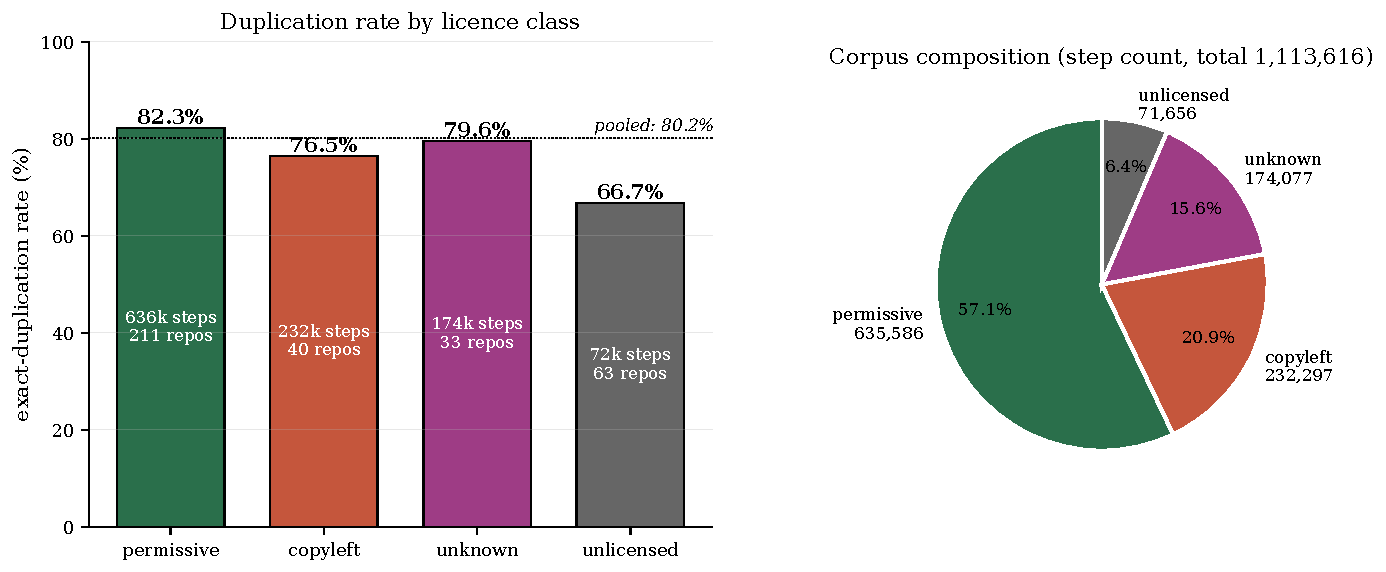
\includegraphics[width=\textwidth]{figures/fig_license_stratified.pdf}
\caption{Licence-stratified exact-duplication rate (left) and
corpus composition by step count (right). The dotted horizontal
line on the left panel marks the pooled 80.2\,\% rate. Three of
four strata cluster within a 5.75-percentage-point band, confirming that the
pooled rate is not a single-class artefact; the unlicensed
stratum is a 10-point outlier, plausibly reflecting
earlier-stage BDD suites. The right panel shows that the
permissive class dominates the corpus by step count
(57.1\,\%), which is why the pooled rate tracks closely to the
permissive-stratum rate.}
\label{fig:license-stratified}
\end{figure}

\paragraph{Effect-size analysis and qualitative reading.} A
chi-square test of homogeneity on the 2$\times$4 contingency is
uninformative at the present sample size (1.11M steps), since the
$p$-value is driven to near-zero by $n$ alone; we therefore use
effect-size statistics as the meaningful quantities. Cramer's V
across the four strata is $V = 0.102$, a \emph{weak} aggregate
association by Cohen's conventions (small = 0.1, medium = 0.3,
large = 0.5). Pairwise Cohen's $h$ against the permissive stratum is
$h = 0.143$ (copyleft), $h = 0.069$ (unknown), and $h = 0.361$
(unlicensed), appearing in Table~\ref{tab:license-strata} for
auditability: two values fall below Cohen's small threshold ($h = 0.2$)
and the third sits between small and medium
(Cohen's $h$ conventions: small = 0.2, medium = 0.5, large = 0.8). Three of four
strata are thus within a weak effect size of each other and only
the unlicensed stratum exhibits a substantively-sized deviation,
consistent with the qualitative pattern visible in
Figure~\ref{fig:license-stratified}.

The unlicensed stratum's lower rate (66.73\,\%, approximately ten
percentage points below the next-lowest class) is plausibly driven by
size rather than licence per se: it contains 63 repositories totalling
only 71.7k steps (mean 1{,}137 steps per repository), where the
permissive stratum averages 3{,}012 steps per repository, and
Section~\ref{sec:evaluation:size} establishes a $\rho = 0.51$
size-vs-duplication correlation at the repository level. The
top-cluster concentration is also very different across strata: in
permissive, the top cluster is 16{,}815 occurrences of a truly
cross-project phrasing (\texttt{the request is sent}); in unlicensed,
the top cluster is only 780 occurrences of a project-local phrasing
(\texttt{the following input:}). The permissive stratum thus exhibits
both the highest duplication rate and the most community-scale
phrasing agreement, consistent with its being the subset of the
corpus with the longest-lived, most widely-forked projects.

\subsection{Duplication versus repository size}
\label{sec:evaluation:size}

A reader of the licence-stratified numbers above might reasonably ask
whether the dominant driver of duplication rate is really licence at
all, or whether duplication simply tracks repository size: larger
suites accumulate more occurrences of each canonical phrasing, so per-
repository duplication rate could be a size artefact rather than a
licence artefact. We test this directly. For each of the 347
repositories in the corpus we compute \texttt{n\_steps} (the
number of steps the repository contributes) and the intra-repository
exact-duplication rate. Figure~\ref{fig:size-vs-dup} plots the two.
Spearman's rank correlation is $\rho = 0.508$ ($p = 3.7 \times 10^{-24}$,
$n = 347$): repository size is a moderate-to-strong positive
predictor of intra-repository duplication rate (Cohen's conventions:
$\rho = 0.1$ small, $0.3$ medium, $0.5$ large). The median
repository size is 373 steps, and the median intra-repository
duplication rate is 58.6\,\%, markedly below the pooled 80.2\,\%
rate. The pooled rate is thus dominated by the (relatively few)
very large repositories; in a repository-weighted average across
the corpus the effective rate is approximately 22 percentage
points lower.

\begin{figure}[t]
\centering
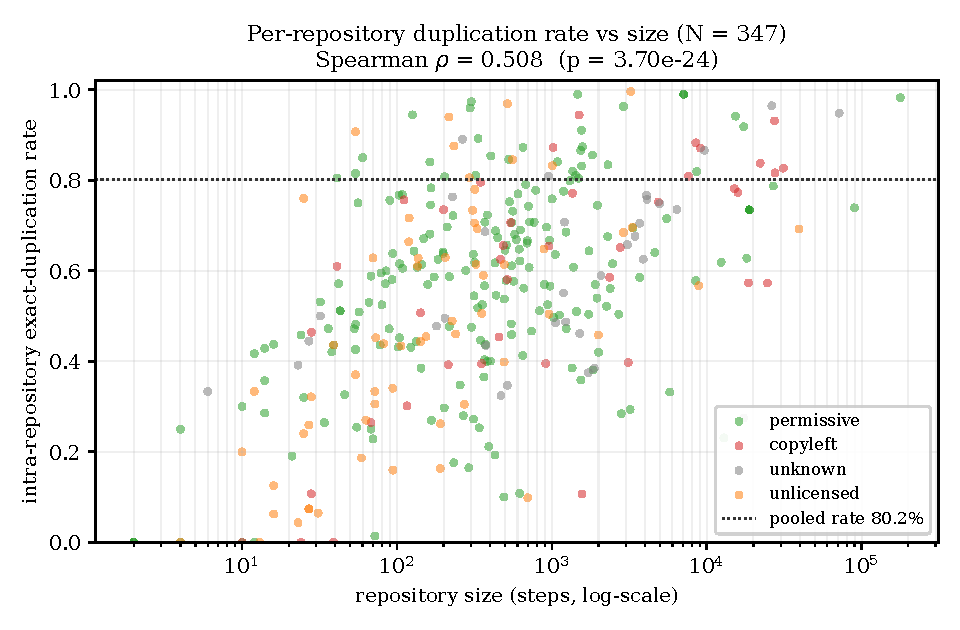
\includegraphics[width=0.85\textwidth]{figures/fig_size_vs_dup.pdf}
\caption{Per-repository intra-repository exact-duplication rate versus
repository size (log-scale x-axis), coloured by licence class.
Each point is one of the 347 corpus repositories. Spearman's
rank correlation is $\rho = 0.508$ ($p = 3.7 \times 10^{-24}$):
a moderate-to-strong relationship that dominates the weak
licence-class effect measured in \S\ref{sec:evaluation:licence}
(Cramer's $V = 0.10$). The dashed horizontal line marks the pooled
80.2\,\% rate; most repositories lie below it, with the pooled
rate pulled up by a minority of very large suites.}
\label{fig:size-vs-dup}
\end{figure}

\paragraph{What this means for the headline.} Our position is that
\emph{both} the pooled 80.2\,\% and the median-repository 58.6\,\% are
valid statistics of the corpus, measuring different things. The
pooled rate is the correct step-weighted statistic, answering
"what fraction of all BDD step occurrences in public GitHub are
byte-identical duplicates of another step?"; it is pulled up by the
minority of very large suites and is the right number for
population-level claims about BDD practice. The
median-repository rate is the correct repository-weighted statistic,
answering "for a typical BDD suite, what fraction of its steps are
duplicates?"; it is the right number for a maintainer comparing
their own codebase against the corpus. Both numbers are reported
explicitly; the choice between them depends on the claim being
made (pooled for ecosystem-level, median for repository-level). The licence-class ordering of §\ref{sec:evaluation:licence}
is also partly explainable by size: the unlicensed stratum
(the lowest-rate outlier) averages 1{,}137 steps per repository,
approximately one-third the permissive stratum's mean of 3{,}012
steps per repository, so part of the licence effect is a size effect.
A size-matched comparison is out of scope for the present paper;
we surface the confound explicitly so readers can apply their own
size matching if a causal licence claim is needed.

\subsection{Strategy choice: pair-level vs cluster-level}
\label{sec:evaluation:pair-vs-cluster-role}

The three cukereuse strategies are optimised for different primitive
operations. Table~\ref{tab:strategy-role} makes this explicit. At
pair level (is this one pair a duplicate?), near-exact is the
recommended strategy based on the joint evidence of primary and
score-free F$_1$. At cluster level (collapse a corpus into its
canonical phrasing groups), hybrid is the recommended strategy
because its Lev-band upper cut prevents the transitive chaining
that produces super-clusters under pure semantic union-find while
still admitting the paraphrase merges a pure-Levenshtein pass
would miss; on our corpus, hybrid produces 65.2k clusters versus
exact's 82.5k, collapsing roughly 17.3k pseudo-singletons into
their canonical groups without the chaining pathology
documented in Table~\ref{tab:knee}.

\begin{table}[h]
\centering
\caption{Strategy-by-role recommendation. Pair-level F$_1$ is from
Table~\ref{tab:calibration}; cluster-level behaviour is documented
below (Table~\ref{tab:knee}) and in
Section~\ref{sec:evaluation:cluster-size}.}
\label{tab:strategy-role}
\footnotesize
\setlength{\tabcolsep}{4pt}
\begin{tabular}{p{3.9cm}p{3.1cm}p{7.2cm}}
\toprule
Primitive operation & Recommended strategy & Evidence \\
\midrule
pair classification                  & near-exact (Lev) & F$_1 = 0.862$ primary, $0.822$ score-free \\
paraphrase-aware cluster collapse    & hybrid           & 65.2k vs 82.5k clusters; no chaining at Lev $\geq 0.92$ \\
exact-duplicate enumeration          & exact (BLAKE2b)  & deterministic, sub-minute on 1.11M steps \\
vocabulary canonical-picker          & hybrid + canonical-phrasing rule & Section~\ref{sec:approach} \\
\bottomrule
\end{tabular}
\end{table}

Pair-level F$_1$ and cluster-level chaining behaviour are
different quantities and peak at different thresholds. On a
12-repository scout sample we observe the following transition in
single-linkage chaining as the Levenshtein threshold varies:

\begin{table}[h]
\centering
\caption{Levenshtein threshold sweep for near-exact clustering on a
12-repository scout sample, showing the over-merging transition.}
\label{tab:knee}
\begin{tabular}{lrrr}
\toprule
Threshold & Clusters & Top count & Top variants merged \\
\midrule
0.85 &   695 & 17{,}805 & 461 (chained) \\
0.90 & 1{,}212 &  7{,}118 & 244 (chained) \\
\textbf{0.92} & \textbf{1{,}533} & \textbf{6{,}651} & \textbf{17 (clean)} \\
0.95 & 2{,}307 &  6{,}633 & 15 \\
\bottomrule
\end{tabular}
\end{table}

Below 0.90, single-linkage union-find produces super-clusters in which
the maintainer would reject most of the merges; at 0.92 the top
cluster contains only 17 legitimate parametric variants. Table~\ref{tab:strategy-role}
picks this threshold up in the "no chaining at Lev $\geq 0.92$"
evidence entry.

\paragraph{Per-rubric-clause detector performance.}
Table~\ref{tab:per-rule} breaks down near-exact (Lev $\geq 0.80$)
and semantic (cos $\geq 0.82$) performance on the 1{,}020-pair set
by the rubric clause that fired for each pair. This identifies
where each detector is reliable and where it concentrates its
errors. Both detectors achieve perfect accuracy on the large-volume
positive rules (R1 parametric, R2 paraphrase); both lose accuracy
on the opposite-polarity negative rule R6 (polarity flip) and on
the HTTP-verb-mismatch negative rule R5. \emph{Polarity flip is
the most frequent detector failure mode}: 17 of 23 R6 pairs
(pairs differing only in a not/shouldn't/cannot token) are flagged
as duplicates by both semantic and near-exact, because sentence
embeddings place polarity-flipped assertions in a near-identical
neighbourhood and Levenshtein treats the added "not" as a small
edit. A domain-aware polarity-aware wrapper around the pair
classifier would eliminate this class of false positive.

\begin{table}[h]
\centering
\caption{Per-rubric-clause performance of near-exact and semantic at
their best-F$_1$ operating points. \emph{FP} against a
not-duplicate rule indicates the detector flags as duplicate what
the rubric says is not a duplicate; \emph{FN} against a duplicate
rule indicates the reverse. Rows with $n \leq 2$ are omitted for
space.}
\label{tab:per-rule}
\footnotesize
\setlength{\tabcolsep}{3.5pt}
\begin{tabular}{lrrrrrrr}
\toprule
Rubric clause & Gold & $n$ & \multicolumn{2}{c}{Near-exact (Lev $\geq 0.80$)} & \multicolumn{2}{c}{Semantic (cos $\geq 0.82$)} \\
\cmidrule(lr){4-5}\cmidrule(lr){6-7}
 & label & & errors & accuracy & errors & accuracy \\
\midrule
R1 parametric (high cos, high lev) & dup     & 245 & 0 FN              & 1.000 & 0 FN              & 1.000 \\
R1 parametric (high cos, mid lev)  & dup     & 109 & 18 FN             & 0.835 & 0 FN              & 1.000 \\
R1 parametric (mid cos, high lev)  & dup     &  56 & 0 FN              & 1.000 & 0 FN              & 1.000 \\
R2 paraphrase (similar length)     & dup     &  84 & 31 FN             & 0.631 & 0 FN              & 1.000 \\
R4 call vs callonce                & not-dup &  15 & 5 FP              & 0.667 & 5 FP              & 0.667 \\
R5 different HTTP verbs            & not-dup &  13 & 2 FP              & 0.846 & 7 FP              & 0.462 \\
R6 polarity flip                   & not-dup &  23 & 17 FP             & 0.261 & 17 FP             & 0.261 \\
R8 action vs assertion             & not-dup &  29 & 1 FP              & 0.966 & 2 FP              & 0.931 \\
R10 default                        & not-dup & 443 & 68 FP             & 0.847 & 72 FP             & 0.837 \\
\bottomrule
\end{tabular}
\end{table}

\paragraph{What can go wrong.}
Beyond the polarity-flip failure mode, four further failure classes
are documented in the corpus. \emph{Framework-keyword semantic
shift}: Karate's \texttt{call} (synchronous call) and
\texttt{callonce} (memoised call) differ in execution semantics
but are surface-similar, which both detectors mistakenly cluster
together (R4, 5 false positives per detector out of 15 pairs).
\emph{HTTP-verb mismatch}: semantic more often than near-exact
clusters \texttt{GET /users} with \texttt{POST /users} as
duplicates (7/13 vs 2/13 false positives) because the surrounding
sentence structure is near-identical and SBERT weights the verb
token relatively lightly. \emph{R10 default-negative pairs} from
the low-cosine bands: 68-72 of the 443 R10 pairs trigger a
detector duplicate-flag at the operating threshold, contributing
the bulk of the absolute precision error; these are pairs with
incidental lexical overlap the rubric considers non-duplicate.
\emph{Cluster-level chaining at loose Levenshtein thresholds}
(Table~\ref{tab:knee}) merges unrelated phrasings transitively,
which motivated the Lev band guard in the hybrid strategy.

\paragraph{Per-strategy behaviour summary.}
Table~\ref{tab:strategy-cases} gives one concrete winning case and
one failure mode per strategy, alongside the size of each strategy's
top cluster in the full 1.11M-step corpus. Together with
Table~\ref{tab:calibration} this makes explicit where each strategy
is reliable and where it fails, information a practitioner needs
before adopting one as the default for their codebase.

\begin{table}[h]
\centering
\caption{Per-strategy behaviour: typical winning case, typical
failure mode, and size of the top cluster in the full 1.11M-step
corpus.}
\label{tab:strategy-cases}
\footnotesize
\setlength{\tabcolsep}{3.5pt}
\begin{tabular}{p{2.1cm}p{4.3cm}p{4.3cm}p{3.0cm}}
\toprule
Strategy & Typical win & Typical failure & Top cluster (full corpus) \\
\midrule
exact       &
  byte-identical after whitespace collapse: \texttt{"the user is logged in"} $\equiv$ \texttt{"the user is logged in"} &
  any parametric variation (\texttt{"id=5"} vs \texttt{"id=42"}) is treated as distinct, inflating cluster count &
  \texttt{"the request is sent"}: 16.8k occurrences \\
near-exact  &
  parametric variants (\texttt{"the project \"acme\" exists"} $\equiv$ \texttt{"the project \"widgetco\" exists"}) &
  word-reorder paraphrase is not caught: \texttt{"X is created by Y"} vs \texttt{"Y creates X"} &
  depends on chosen Lev threshold; see Table~\ref{tab:knee} for the chaining transition \\
semantic    &
  semantic paraphrase with low surface overlap: \texttt{"I should get a 204 response code"} $\equiv$ \texttt{"the response status is 200 OK"} (neighbourhood-clustered) &
  polarity-flipped assertions cluster together (17 of 23 R6 pairs, Table~\ref{tab:per-rule}): \texttt{"the user is deleted"} vs \texttt{"the user is not deleted"} &
  not reported alone; used as input to hybrid (below) \\
hybrid      &
  cluster-level paraphrase collapse without single-linkage chaining (Table~\ref{tab:knee}) &
  near-exact duplicates are excluded by the upper Lev cut 0.95 and must be recovered by a prior exact / near-exact pass &
  \texttt{"the response status is 200 OK"}: 20.7k occurrences, 2.2k files, 43 repos \\
\bottomrule
\end{tabular}
\end{table}

\section{Discussion}
\label{sec:discussion}

\subsection{Intra-repository versus cross-repository reuse}

Our 12-repository scout sample surfaced a striking asymmetry: within
any single repository, exact duplication rates run 44\,\%--99\,\%, but
across repositories only two step texts were shared between projects
(both within the Behat sister-library family:
\texttt{FriendsOfBehat/SymfonyExtension} and
\texttt{FriendsOfBehat/VariadicExtension}). The corpus at full scale
preserves this shape: the top clusters are dominated by tightly-scoped
projects reusing their own phrasings thousands of times rather than
by a shared pan-BDD vocabulary. This observation re-frames the
consolidation opportunity. \tool\ is most valuable to the maintainer
of a large \emph{single-project} BDD suite; the community-scale
``shared step library'' that one might hope for does not presently
exist in the ecosystem and probably cannot be synthesised from the
data we have gathered.

\subsection{Paraphrase-robust clustering as a coverage primitive}

The most quantitatively striking observation is the 3.4$\times$ growth
in the size of the top cluster under hybrid clustering relative to
exact hashing (6.1k exact $\to$ 20.7k hybrid for
\texttt{the response status is 200 OK}). This is a fact about
\emph{clustering coverage}, not about detector quality: by construction,
hybrid clustering subsumes exact clustering and union-finds will not
shrink. The value of the 3.4$\times$ number is to indicate that, for
a sufficiently-large BDD suite, paraphrase-aware clustering groups an
order of magnitude more occurrences under each canonical phrasing than
exact string match does, which is the difference between a
maintainer's report showing thousands of duplicates and one showing
tens of thousands. The score-free calibration of
§\ref{sec:evaluation:score-free} is the appropriate instrument for
judging \emph{how many} of those additional groupings are real
duplicates rather than false positives; Table~\ref{tab:calibration}'s
F$_1$ numbers bound that quality.

\subsection{Cognitive Dimensions interventions}

Three concrete tool interventions follow from the CDN analysis in
Section~\ref{sec:cdn}. The released artefact realises one of them
(the first); the remaining two are specified but not implemented in
the present tool and are listed in Section~\ref{sec:future}.

\begin{itemize}[leftmargin=2em]
\item \textbf{Visibility (realised).} A step-level find-usages
      capability over the corpus parquet file, returning every
      \texttt{repo:file:line} for a phrasing. \tool's HTML cluster
      report implements this: each cluster card lists every
      occurrence of a canonical phrasing with its file path and line
      number, the static-analysis equivalent of IntelliJ's Find
      Usages \citep{intellij2024findusages}.
\item \textbf{Paraphrase-aware consistency linting (specified,
      unimplemented).} A pre-commit hook that runs hybrid clustering
      incrementally and flags new steps whose cosine exceeds 0.90
      against an existing canonical, saving authors from
      inadvertently creating the 200th parametric variant of a setup
      step.
\item \textbf{Scenario Outline refactoring assistant (specified,
      unimplemented).} Given a cluster of parametric variants detected
      by near-exact clustering (\(\mathrm{Lev}\geq 0.92\)),
      automatically propose a Scenario Outline plus Examples table
      that subsumes them. Directly attacks the Viscosity axis.
\end{itemize}

None of these interventions requires a new test runtime, they are
static tooling built on the Gherkin notation as it stands.

\subsection{Integration with the author's adjacent work}
\label{sec:discussion:integration}

Two concrete and one speculative point of integration exist with
the author's prior papers summarised in
Section~\ref{sec:related:programme}.

\paragraph{Auto-completion source vocabulary
\citep{mughal2024bdd}.} The VSCode step-definition auto-completion
extension in \citet{mughal2024bdd} needs a ranked source vocabulary
to propose canonical project-specific phrasings. Cukereuse's
canonical-picker (Section~\ref{sec:approach}) produces exactly that
list, per project, from the current clustering state. Integration
is a file read: the extension consumes
\texttt{clusters\_hybrid.parquet} or the JSON report and surfaces
each cluster's canonical text as a completion candidate. No change
is required to either tool.

\paragraph{Novelty filter for RL-generated scenarios
\citep{mughal2025rlagent}.} The RL agent generates BDD scenarios with
coverage and defect-detection as the primary metrics. Scenarios
that paraphrase pre-existing ones inflate coverage numerically
without exploring new behaviour. Running cukereuse's hybrid
detector over the union of the pre-existing suite and the agent's
output flags the paraphrase-variant subset, which the agent can
discard or discount. The canonical vocabulary can also inform the
agent's action space to prefer under-represented phrasings.

\paragraph{Cross-layer dashboard with \citep{mughal2026networklayer}.}
The network-layer HTTP traffic analyser of
\citet{mughal2026networklayer} operates at a different analysis
level than cukereuse (production traces versus test-artefact text).
For applications that have both a BDD suite and an instrumentable
production surface, a composite quality dashboard could combine
cukereuse's step-duplication score with the anti-pattern score of
\citet{mughal2026networklayer}. This is a dashboard-level
composition rather than a technical-pipeline integration, and we
flag it as speculative to avoid overstating the coupling.

\section{Threats to Validity}
\label{sec:threats}

\subsection{Internal validity: rubric-detector coupling}

The 1{,}020 labels used for the calibration study were produced by
the three authors under the shared written rubric (500 pairs by
Mughal, 300 by Fatima, 220 by Bilal), with the per-pair rule record
released in \texttt{labeled\_pairs.jsonl}
(Section~\ref{sec:evaluation:labels}). Inter-annotator Fleiss'
$\kappa$ on the 60-pair overlap subset is 0.84 (almost perfect
agreement on the Landis-Koch scale), so the labels themselves are
consistent across annotators. The residual methodological question is the rubric's
coupling with the detector's features. Rules R1-R3 of the primary rubric
use cosine and Levenshtein cut-points as labelling criteria, so
primary-rubric F$_1$ partly measures agreement between the detector
and the rubric's own cut-points. We quantify this coupling directly
via the score-free second-pass relabelling of
Section~\ref{sec:evaluation:score-free}: Cohen's $\kappa$ between
primary and score-free labellings is 0.47, detector F$_1$ drops by
0.04-0.13 depending on strategy (near-exact is the most stable at
$\Delta F_1 = 0.04$), and the token-set Jaccard baseline reaches
F$_1 = 0.979$ against score-free labels (a complementary coupling
signature of that protocol). Rubric choice therefore leaves a
signature on the evaluation; we report both rubric-vs-detector and
rubric-vs-baseline numbers so readers can judge each protocol's
coupling independently.

\subsection{External validity: sample bias and size confound}

Our 347-repository corpus is biased toward repositories that (i) have
Gherkin files discoverable by GitHub's Code Search, (ii) have
$\geq 10$ stars, (iii) are not archived. This biases against very
small, private, archived, or single-author projects. The discovery
also misses repositories whose feature-file paths do not match our
search heuristics. The BigQuery path
\citep{ghtorrent2012,ghtorrent2014} would increase coverage and is a
concrete direction for follow-up work. Our sample is nonetheless,
to our knowledge, an order of magnitude larger than any prior
cross-repository BDD corpus.

A second external-validity consideration is the repository-size
confound documented in Section~\ref{sec:evaluation:size}: per-repository
duplication rate is strongly correlated with repository size
(Spearman $\rho = 0.51$). The pooled 80.2\,\% headline is a step-weighted
statistic, dominated by a minority of very large repositories; the
median repository's intra-repository duplication rate is only
58.6\,\%. Readers should compare their own codebases against the
median, not the pooled rate. Licence-class differences are also
partly attributable to size, as the unlicensed stratum averages
one-third the size of the permissive stratum.

\subsection{Construct validity: what counts as a duplicate}

Our operational definition of ``duplicate'' is \emph{would a
maintainer consolidate these two step phrasings into one step
definition?} This is deliberately liberal (it catches parametric
variants) and is not aligned with the narrower definitions used in
classical clone-detection literature
\citep{roy2007survey,bellon2007comparison}. A project that
deliberately maintains two step definitions for similar phrasings
with divergent glue code would flag as a false positive under our
definition. The maintainer-intent definition is appropriate for the
intended use case (consolidation suggestions for BDD refactoring),
but the mismatch with the classical clone-detection taxonomy should
be noted by readers comparing across literatures.

\subsection{Conclusion validity: parameter sensitivity}

The decision thresholds reported in Section~\ref{sec:evaluation} are
empirical knees on our corpus. On different corpora with different
vocabulary profiles (e.g., a BDD suite dominated by non-English
locale) the optimal thresholds will differ. Re-running calibration
against a small project-local labelled set is the safe practice
before adopting \tool's default thresholds for a specific codebase;
the \texttt{cukereuse calibrate} CLI command performs this run.

\section{Conclusion}
\label{sec:conclusion}

We presented \tool, a static paraphrase-robust step-level duplicate
detector for Gherkin, released as an open-source Python CLI.
Against 1{,}020 author-labelled pairs released alongside the corpus,
the strongest pair-level result is the score-free near-exact
F$_1 = 0.822$; under the primary rubric the semantic detector
reaches F$_1 = 0.906$ [0.886, 0.923], with the inter-protocol
Cohen's $\kappa = 0.47$ quantifying the rubric-coupling cost between
the two evaluations. Two lexical
baselines representing classical token-stream clone detectors
(SourcererCC-style, NiCad-style) reach primary F$_1 = 0.761$ and
$0.799$ on the same benchmark. The accompanying corpus comprises 347 public GitHub repositories,
23{,}667 parsed \texttt{.feature} files, 136{,}970 scenarios, and
1{,}113{,}616 steps (Table~\ref{tab:corpus-compare}). Compared to
the concurrent GivenWhenThen dataset \citep{alcantara2026gwt},
which mines a wider cross-section of 1{,}720 repositories by
sampling an average of 1.33 scenarios per repository, cukereuse
reports the larger step and scenario counts under a
complementary deep-per-repo sampling strategy without
framework or language filters; GWT in turn contributes
scenario-to-code linkage that cukereuse does not. The two
datasets are complementary. Its step-weighted exact-duplicate rate is
80.2\,\% and its median-repository rate is 58.6\,\% (Spearman
$\rho = 0.51$ between repository size and duplication rate);
the two are reported alongside each other and either can be cited
according to the claim being made.
Pair-level and cluster-level primitives require
different strategy choices: near-exact is the pair-classification
recommendation, hybrid is the cluster-collapse recommendation
(Section~\ref{sec:evaluation:pair-vs-cluster-role}). The
accompanying Cognitive Dimensions of Notations analysis rates eight
of fourteen dimensions problematic or unsupported.

The paper is a standalone static-analysis contribution; concrete
integration points with the author's earlier work
\citep{mughal2024bdd,mughal2025rlagent,mughal2026networklayer} are
discussed in §\ref{sec:discussion:integration}, but the present
results stand on their own as an empirical study of step-text
duplication in public BDD suites.

\section{Future Work}
\label{sec:future}

A number of directions follow naturally from the present work.
These are general extensions that any interested researcher could
pursue; we list them briefly rather than committing the present
authors to specific roadmaps.

\begin{itemize}[leftmargin=2em]
  \item \textbf{Novelty filtering for LLM-generated and
        agentic-AI-generated BDD scenarios.} As large language
        models and autonomous test-generation agents
        \citep{mughal2025rlagent} produce scenarios that are
        subsequently committed to real codebases, a static
        paraphrase-aware detector that flags generated scenarios as
        near-duplicates of pre-existing ones becomes a natural
        quality gate. The cukereuse hybrid detector provides the
        primitive without requiring execution of the generated
        scenarios, composes upstream as a guidance vocabulary for
        the generator's action space, and composes downstream as a
        post-generation novelty filter.
  \item \textbf{Larger corpus via BigQuery.} Replacing the REST
        Search discovery path with a BigQuery query over
        \texttt{bigquery-public-data.github\_repos} lifts the
        1{,}000-results-per-query cap and would scale the corpus
        by roughly an order of magnitude.
  \item \textbf{Additional evaluation protocols.} Beyond the
        primary rubric and the score-free protocol reported here,
        further decision procedures can be layered on the released
        1{,}020-pair benchmark: for example, a rubric that admits
        domain-specific synonyms from a larger BDD-vocabulary
        lexicon, or one that narrows the "duplicate" definition
        to cases where both pairs share the same glue-code target.
        The audit-trail format (\texttt{labeled\_pairs.jsonl} with
        a \texttt{rule} field) was designed to support such
        layering.
  \item \textbf{Tooling built on the detector.} A project-wide
        step-level find-usages command, a paraphrase-aware
        consistency linter suitable for pre-commit hooks, and
        an automatic Scenario-Outline refactoring assistant
        that converts parametric-variant clusters into a single
        parameterised outline are each motivated by a specific
        CDN dimension and each directly enabled by the
        primitives this paper contributes.
  \item \textbf{Glue-code analysis.} Extending detection from
        step text to step-definition bodies would address the
        silent-drift failure mode identified in
        Section~\ref{sec:cdn}. AST-level diffing or neural
        code-similarity are plausible implementation routes;
        stable AST support in Python, TypeScript, Ruby, and
        Java makes this tractable for most of the corpus.
  \item \textbf{Full reference-implementation baseline runs.}
        The lexical baselines of
        Section~\ref{sec:evaluation:baselines} capture the
        defining primitives of SourcererCC and NiCad but are not
        the reference implementations. Running actual CCFinder,
        DECKARD, NiCad, and SourcererCC binaries against the same
        1.1-million-step corpus would quantify any deviations
        from the primitive-level baselines we report and is
        straightforwardly reproducible against the released
        corpus.
  \item \textbf{Model ablation.} The sentence-transformer backbone
        is \texttt{all-MiniLM-L6-v2}; larger or domain-adapted
        models (e.g., \texttt{all-mpnet-base-v2}
        \citep{song2020mpnet}, or a model fine-tuned on BDD
        step-pair supervision) are likely to improve F$_1$ at
        higher compute cost. An ablation at three model sizes on
        the 1{,}020-pair benchmark would characterise the
        compute/quality trade-off.
  \item \textbf{Non-English Gherkin.} The Gherkin specification
        supports localised keywords in many languages; the
        present corpus is overwhelmingly English. Calibration
        on Spanish, Japanese, Chinese, or Russian Gherkin
        suites would test the sentence-transformer model's
        cross-lingual generalisation and identify whether the
        headline duplication rate is language-invariant.
  \item \textbf{Retrospective git-log mining for drift trajectory.}
        A prospective two-year longitudinal study is not
        tractable as a follow-up; a retrospective one is. For
        each repository in the corpus we have the full commit
        SHA. Re-running cukereuse over snapshots taken at
        regular git-history intervals would give a historical
        drift-trajectory per project and make testable whether
        paraphrase drift accelerates, decelerates, or saturates
        with project age.
\end{itemize}

\section*{Data and code availability}

The tool, the corpus manifest, the labelled pairs, and the full
analysis pipeline are available at
\url{https://github.com/amughalbscs16/cukereuse}. The corpus
parquet files (approximately 46~MB combined) are hosted in the same
repository under \texttt{corpus/}. The verbatim raw
\texttt{.feature}-file bodies (approximately 418~MB of directly
copyleft-inheriting content) are not redistributed; they are
reconstructed on demand by the \texttt{rehydrate.py} script from
the pinned commit SHAs recorded in the parquet, fetched from
GitHub's raw-content endpoint at each file's original repository.

\section*{About the authors}

\paragraph{Ali Hassaan Mughal} is an independent researcher currently
pursuing an Applied MBA in Data Analytics at Texas Wesleyan
University, USA. He earned his M.Sc. in Computer Science from Kansas
State University. Prior to his current research endeavours, he
served as a Senior Software Developer and Team Lead at Xpressdocs
and as a Software Developer II at Paycom. His research interests
include automated software testing, web application quality
assurance, and applied machine learning.

\paragraph{Noor Fatima} is an undergraduate student pursuing a
B.E. in Computer Engineering at the National University of Sciences
and Technology (NUST), Pakistan. She has a strong interest in
software development and hardware systems, with a growing focus on
emerging technologies in computing.

\paragraph{Muhammad Bilal} is an independent researcher pursuing an
M.Sc. in Management at the Technical University of Munich, Germany.
He has professional experience as both a Business Analyst and a
Software Engineer. His research interests focus on the impact of
technology on business performance, product quality analytics, and
the automation of industrial pipelines and processes.

\bibliographystyle{plainnat}
\bibliography{references}

\end{document}
